\hypertarget{group__dbprim__rbtree}{
\section{Red-black trees}
\label{group__dbprim__rbtree}\index{Red-black trees@{Red-black trees}}
}


\subsection{Detailed Description}
Red-black trees are a form of binary search tree. One essential feature of binary search trees is that they need to be balanced in order to be efficient. Many algorithms exist for keeping trees balanced, but among the easiest to implement is the red-black tree. In a red-black tree, every node is given a color--either red or black--and there are various rules for what color nodes can be present where in the tree. This library implements these rules, along with functions for traversing the tree in any desired tree order.

A red-black tree is represented by a caller-allocated \hyperlink{group__dbprim__rbtree_ga0}{rb\_\-tree\_\-t} structure. This structure describes various characteristics of the tree, such as the number of nodes in the tree, and includes a pointer to the root node of the tree. Nodes may be added to the tree using \hyperlink{group__dbprim__rbtree_ga7}{rt\_\-add()} or removed from the tree using \hyperlink{group__dbprim__rbtree_ga9}{rt\_\-remove()}. Additionally, the key on a given node may be changed using the \hyperlink{group__dbprim__rbtree_ga8}{rt\_\-move()} function. Nodes may be looked up with \hyperlink{group__dbprim__rbtree_ga10}{rt\_\-find()}, and \hyperlink{group__dbprim__rbtree_ga12}{rt\_\-iter()} will execute a user-defined function for each node in the tree in the specified order. To remove all entries in the tree, simply call the \hyperlink{group__dbprim__rbtree_ga13}{rt\_\-flush()} function. If you must manually iterate through the tree, you may call the \hyperlink{group__dbprim__rbtree_ga11}{rt\_\-next()} and \hyperlink{group__dbprim__rbtree_ga29}{rt\_\-prev()} functions to determine the next or previous nodes to visit.

There are three ways to traverse a binary tree. The first, known as \char`\"{}preorder,\char`\"{} visits the root node, then traverses the left subtree in preorder, then traverses the right subtree in preorder. The second, known an \char`\"{}inorder,\char`\"{} traverses the left subtree in inorder, then the root node, then the right subtree in inorder. (This particular ordering retrieves the nodes in lexical order; thus its name.) The third ordering is known as \char`\"{}postorder\char`\"{}; this ordering traverses the left subtree, the right subtree, then visits the root node. To iterate over the tree in one of these orderings, simply call \hyperlink{group__dbprim__rbtree_ga12}{rt\_\-iter()} (or \hyperlink{group__dbprim__rbtree_ga11}{rt\_\-next()} or \hyperlink{group__dbprim__rbtree_ga29}{rt\_\-prev()}) with the \hyperlink{group__dbprim__rbtree_ga25}{RBT\_\-ORDER\_\-PRE}, \hyperlink{group__dbprim__rbtree_ga26}{RBT\_\-ORDER\_\-IN}, or \hyperlink{group__dbprim__rbtree_ga27}{RBT\_\-ORDER\_\-POST} flags. You may OR these flags with \hyperlink{group__dbprim_ga4}{DB\_\-FLAG\_\-REVERSE} to reverse the traversal ordering, if you wish.

\subsection*{Data Structures}
\begin{CompactItemize}
\item 
struct \hyperlink{struct__rb__tree__s}{\_\-rb\_\-tree\_\-s}
\begin{CompactList}\small\item\em Red-black tree structure. \item\end{CompactList}\item 
struct \hyperlink{struct__rb__node__s}{\_\-rb\_\-node\_\-s}
\begin{CompactList}\small\item\em Red-black tree node structure. \item\end{CompactList}\end{CompactItemize}
\subsection*{Defines}
\begin{CompactItemize}
\item 
\#define \hyperlink{group__dbprim__rbtree_ga17}{RB\_\-TREE\_\-MAGIC}
\begin{CompactList}\small\item\em Red-black tree magic number. \item\end{CompactList}\item 
\#define \hyperlink{group__dbprim__rbtree_ga18}{RB\_\-TREE\_\-INIT}(comp, extra)
\begin{CompactList}\small\item\em Red-black tree static initializer. \item\end{CompactList}\item 
\#define \hyperlink{group__dbprim__rbtree_ga19}{rt\_\-verify}(tree)
\begin{CompactList}\small\item\em Red-black tree verification macro. \item\end{CompactList}\item 
\#define \hyperlink{group__dbprim__rbtree_ga20}{rt\_\-frozen}(tree)
\begin{CompactList}\small\item\em Determine if a red-black tree is frozen. \item\end{CompactList}\item 
\#define \hyperlink{group__dbprim__rbtree_ga21}{rt\_\-count}(tree)
\begin{CompactList}\small\item\em Red-black tree count. \item\end{CompactList}\item 
\#define \hyperlink{group__dbprim__rbtree_ga22}{rt\_\-root}(tree)
\begin{CompactList}\small\item\em Red-black tree root node. \item\end{CompactList}\item 
\#define \hyperlink{group__dbprim__rbtree_ga23}{rt\_\-comp}(tree)
\begin{CompactList}\small\item\em Red-black tree comparison function. \item\end{CompactList}\item 
\#define \hyperlink{group__dbprim__rbtree_ga24}{rt\_\-extra}(tree)
\begin{CompactList}\small\item\em Extra pointer data in a red-black tree. \item\end{CompactList}\item 
\#define \hyperlink{group__dbprim__rbtree_ga25}{RBT\_\-ORDER\_\-PRE}
\begin{CompactList}\small\item\em Preorder tree traversal method. \item\end{CompactList}\item 
\#define \hyperlink{group__dbprim__rbtree_ga26}{RBT\_\-ORDER\_\-IN}
\begin{CompactList}\small\item\em Inorder tree traversal method. \item\end{CompactList}\item 
\#define \hyperlink{group__dbprim__rbtree_ga27}{RBT\_\-ORDER\_\-POST}
\begin{CompactList}\small\item\em Postorder tree traversal method. \item\end{CompactList}\item 
\#define \hyperlink{group__dbprim__rbtree_ga28}{RBT\_\-ORDER\_\-MASK}
\begin{CompactList}\small\item\em Tree traversal method mask. \item\end{CompactList}\item 
\#define \hyperlink{group__dbprim__rbtree_ga29}{rt\_\-prev}(tree, node\_\-io, flags)
\begin{CompactList}\small\item\em Get the previous node. \item\end{CompactList}\item 
\#define \hyperlink{group__dbprim__rbtree_ga30}{RB\_\-NODE\_\-MAGIC}
\begin{CompactList}\small\item\em Red-black tree node magic number. \item\end{CompactList}\item 
\#define \hyperlink{group__dbprim__rbtree_ga31}{RB\_\-NODE\_\-INIT}(value)
\begin{CompactList}\small\item\em Red-black tree node static initializer. \item\end{CompactList}\item 
\#define \hyperlink{group__dbprim__rbtree_ga32}{rn\_\-verify}(node)
\begin{CompactList}\small\item\em Red-black tree node verification macro. \item\end{CompactList}\item 
\#define \hyperlink{group__dbprim__rbtree_ga33}{rn\_\-color}(node)
\begin{CompactList}\small\item\em Red-black tree node color. \item\end{CompactList}\item 
\#define \hyperlink{group__dbprim__rbtree_ga34}{rn\_\-tree}(node)
\begin{CompactList}\small\item\em Red-black tree node's tree pointer. \item\end{CompactList}\item 
\#define \hyperlink{group__dbprim__rbtree_ga35}{rn\_\-parent}(node)
\begin{CompactList}\small\item\em Red-black tree node's parent pointer. \item\end{CompactList}\item 
\#define \hyperlink{group__dbprim__rbtree_ga36}{rn\_\-left}(node)
\begin{CompactList}\small\item\em Red-black tree node's left pointer. \item\end{CompactList}\item 
\#define \hyperlink{group__dbprim__rbtree_ga37}{rn\_\-right}(node)
\begin{CompactList}\small\item\em Red-black tree node's right pointer. \item\end{CompactList}\item 
\#define \hyperlink{group__dbprim__rbtree_ga38}{rn\_\-key}(node)
\begin{CompactList}\small\item\em Red-black tree node's key pointer. \item\end{CompactList}\item 
\#define \hyperlink{group__dbprim__rbtree_ga39}{rn\_\-value}(node)
\begin{CompactList}\small\item\em Red-black tree node's value pointer. \item\end{CompactList}\item 
\#define \hyperlink{group__dbprim__rbtree_ga40}{rn\_\-isblack}(node)
\begin{CompactList}\small\item\em Test if a given node is black. \item\end{CompactList}\item 
\#define \hyperlink{group__dbprim__rbtree_ga41}{rn\_\-isred}(node)
\begin{CompactList}\small\item\em Test if a given node is red. \item\end{CompactList}\item 
\#define \hyperlink{group__dbprim__rbtree_ga42}{rn\_\-isleft}(node)
\begin{CompactList}\small\item\em Test if a given node is the left node of its parent. \item\end{CompactList}\item 
\#define \hyperlink{group__dbprim__rbtree_ga43}{rn\_\-isright}(node)
\begin{CompactList}\small\item\em Test if a given node is the right node of its parent. \item\end{CompactList}\item 
\#define \hyperlink{group__dbprim__rbtree_ga44}{uncle}(node)
\begin{CompactList}\small\item\em Locate the uncle of a node. \item\end{CompactList}\item 
\#define \hyperlink{group__dbprim__rbtree_ga45}{flip}(node)
\begin{CompactList}\small\item\em Flip the color of a node. \item\end{CompactList}\item 
\#define \hyperlink{group__dbprim__rbtree_ga46}{\_\-rn\_\-clear}(node)
\begin{CompactList}\small\item\em Clear a node. \item\end{CompactList}\item 
\#define \hyperlink{group__dbprim__rbtree_ga47}{\_\-rt\_\-update\_\-parent}(tree, node, new)
\begin{CompactList}\small\item\em Update a node's parent. \item\end{CompactList}\item 
\#define \hyperlink{group__dbprim__rbtree_ga48}{isleft}(par, n)
\begin{CompactList}\small\item\em Determine if node is a left child of its parent. \item\end{CompactList}\item 
\#define \hyperlink{group__dbprim__rbtree_ga49}{sel\_\-lr}(t, n)
\begin{CompactList}\small\item\em Select a child node based on a condition. \item\end{CompactList}\item 
\#define \hyperlink{group__dbprim__rbtree_ga50}{sibling}(par, n)
\begin{CompactList}\small\item\em Locate the sibling of a node. \item\end{CompactList}\item 
\#define \hyperlink{group__dbprim__rbtree_ga51}{l\_\-neph}(par, n)
\begin{CompactList}\small\item\em Locate \char`\"{}closer\char`\"{} nephew of a node. \item\end{CompactList}\item 
\#define \hyperlink{group__dbprim__rbtree_ga52}{r\_\-neph}(par, n)
\begin{CompactList}\small\item\em Locate \char`\"{}further\char`\"{} nephew of a node. \item\end{CompactList}\end{CompactItemize}
\subsection*{Typedefs}
\begin{CompactItemize}
\item 
typedef \hyperlink{struct__rb__tree__s}{\_\-rb\_\-tree\_\-s} \hyperlink{group__dbprim__rbtree_ga0}{rb\_\-tree\_\-t}
\begin{CompactList}\small\item\em Red-black tree. \item\end{CompactList}\item 
typedef \hyperlink{struct__rb__node__s}{\_\-rb\_\-node\_\-s} \hyperlink{group__dbprim__rbtree_ga1}{rb\_\-node\_\-t}
\begin{CompactList}\small\item\em Red-black tree node. \item\end{CompactList}\item 
typedef unsigned long($\ast$ \hyperlink{group__dbprim__rbtree_ga2}{rb\_\-iter\_\-t} )(\hyperlink{struct__rb__tree__s}{rb\_\-tree\_\-t} $\ast$tree, \hyperlink{struct__rb__node__s}{rb\_\-node\_\-t} $\ast$node, void $\ast$extra)
\begin{CompactList}\small\item\em Red-black tree iteration callback. \item\end{CompactList}\item 
typedef long($\ast$ \hyperlink{group__dbprim__rbtree_ga3}{rb\_\-comp\_\-t} )(\hyperlink{struct__rb__tree__s}{rb\_\-tree\_\-t} $\ast$tree, \hyperlink{struct__db__key__s}{db\_\-key\_\-t} $\ast$key1, \hyperlink{struct__db__key__s}{db\_\-key\_\-t} $\ast$key2)
\begin{CompactList}\small\item\em Red-black tree comparison callback. \item\end{CompactList}\item 
typedef enum \hyperlink{group__dbprim__rbtree_ga53}{\_\-rb\_\-color\_\-e} \hyperlink{group__dbprim__rbtree_ga4}{rb\_\-color\_\-t}
\begin{CompactList}\small\item\em Red-black tree node color. \item\end{CompactList}\end{CompactItemize}
\subsection*{Enumerations}
\begin{CompactItemize}
\item 
enum \hyperlink{group__dbprim__rbtree_ga53}{\_\-rb\_\-color\_\-e} \{ \hyperlink{group__dbprim__rbtree_gga53a139}{RB\_\-COLOR\_\-NONE}, 
\hyperlink{group__dbprim__rbtree_gga53a140}{RB\_\-COLOR\_\-RED}, 
\hyperlink{group__dbprim__rbtree_gga53a141}{RB\_\-COLOR\_\-BLACK}
 \}
\begin{CompactList}\small\item\em Red-black tree node color. \item\end{CompactList}\end{CompactItemize}
\subsection*{Functions}
\begin{CompactItemize}
\item 
long \hyperlink{group__dbprim__rbtree_ga5}{rbtree\_\-comp} (\hyperlink{struct__rb__tree__s}{rb\_\-tree\_\-t} $\ast$tree, \hyperlink{struct__db__key__s}{db\_\-key\_\-t} $\ast$key1, \hyperlink{struct__db__key__s}{db\_\-key\_\-t} $\ast$key2)
\begin{CompactList}\small\item\em Red-black tree comparison function. \item\end{CompactList}\item 
unsigned long \hyperlink{group__dbprim__rbtree_ga6}{rt\_\-init} (\hyperlink{struct__rb__tree__s}{rb\_\-tree\_\-t} $\ast$tree, \hyperlink{group__dbprim__rbtree_ga3}{rb\_\-comp\_\-t} comp, void $\ast$extra)
\begin{CompactList}\small\item\em Dynamically initialize a red-black tree. \item\end{CompactList}\item 
unsigned long \hyperlink{group__dbprim__rbtree_ga7}{rt\_\-add} (\hyperlink{struct__rb__tree__s}{rb\_\-tree\_\-t} $\ast$tree, \hyperlink{struct__rb__node__s}{rb\_\-node\_\-t} $\ast$node, \hyperlink{struct__db__key__s}{db\_\-key\_\-t} $\ast$key)
\begin{CompactList}\small\item\em Add a node to a red-black tree. \item\end{CompactList}\item 
unsigned long \hyperlink{group__dbprim__rbtree_ga8}{rt\_\-move} (\hyperlink{struct__rb__tree__s}{rb\_\-tree\_\-t} $\ast$tree, \hyperlink{struct__rb__node__s}{rb\_\-node\_\-t} $\ast$node, \hyperlink{struct__db__key__s}{db\_\-key\_\-t} $\ast$key)
\begin{CompactList}\small\item\em Move a node in a red-black tree. \item\end{CompactList}\item 
unsigned long \hyperlink{group__dbprim__rbtree_ga9}{rt\_\-remove} (\hyperlink{struct__rb__tree__s}{rb\_\-tree\_\-t} $\ast$tree, \hyperlink{struct__rb__node__s}{rb\_\-node\_\-t} $\ast$node)
\begin{CompactList}\small\item\em Remove a node from a red-black tree. \item\end{CompactList}\item 
unsigned long \hyperlink{group__dbprim__rbtree_ga10}{rt\_\-find} (\hyperlink{struct__rb__tree__s}{rb\_\-tree\_\-t} $\ast$tree, \hyperlink{struct__rb__node__s}{rb\_\-node\_\-t} $\ast$$\ast$node\_\-p, \hyperlink{struct__db__key__s}{db\_\-key\_\-t} $\ast$key)
\begin{CompactList}\small\item\em Find an entry in a red-black table. \item\end{CompactList}\item 
unsigned long \hyperlink{group__dbprim__rbtree_ga11}{rt\_\-next} (\hyperlink{struct__rb__tree__s}{rb\_\-tree\_\-t} $\ast$tree, \hyperlink{struct__rb__node__s}{rb\_\-node\_\-t} $\ast$$\ast$node\_\-io, unsigned long flags)
\begin{CompactList}\small\item\em Get the next node. \item\end{CompactList}\item 
unsigned long \hyperlink{group__dbprim__rbtree_ga12}{rt\_\-iter} (\hyperlink{struct__rb__tree__s}{rb\_\-tree\_\-t} $\ast$tree, \hyperlink{struct__rb__node__s}{rb\_\-node\_\-t} $\ast$start, \hyperlink{group__dbprim__rbtree_ga2}{rb\_\-iter\_\-t} iter\_\-func, void $\ast$extra, unsigned long flags)
\begin{CompactList}\small\item\em Iterate over each entry in a red-black tree. \item\end{CompactList}\item 
unsigned long \hyperlink{group__dbprim__rbtree_ga13}{rt\_\-flush} (\hyperlink{struct__rb__tree__s}{rb\_\-tree\_\-t} $\ast$tree, \hyperlink{group__dbprim__rbtree_ga2}{rb\_\-iter\_\-t} flush\_\-func, void $\ast$extra)
\begin{CompactList}\small\item\em Flush a red-black tree. \item\end{CompactList}\item 
unsigned long \hyperlink{group__dbprim__rbtree_ga14}{rn\_\-init} (\hyperlink{struct__rb__node__s}{rb\_\-node\_\-t} $\ast$node, void $\ast$value)
\begin{CompactList}\small\item\em Dynamically initialize a red-black tree node. \item\end{CompactList}\item 
\hyperlink{struct__rb__node__s}{rb\_\-node\_\-t} $\ast$ \hyperlink{group__dbprim__rbtree_ga15}{\_\-rb\_\-locate} (\hyperlink{struct__rb__tree__s}{rb\_\-tree\_\-t} $\ast$tree, \hyperlink{struct__rb__node__s}{rb\_\-node\_\-t} $\ast$node, \hyperlink{struct__db__key__s}{db\_\-key\_\-t} $\ast$key)
\begin{CompactList}\small\item\em Locate or insert a red-black tree node. \item\end{CompactList}\item 
void \hyperlink{group__dbprim__rbtree_ga16}{\_\-rb\_\-rotate} (\hyperlink{struct__rb__tree__s}{rb\_\-tree\_\-t} $\ast$tree, \hyperlink{struct__rb__node__s}{rb\_\-node\_\-t} $\ast$child)
\begin{CompactList}\small\item\em Rotate tree nodes. \item\end{CompactList}\end{CompactItemize}


\subsection{Define Documentation}
\hypertarget{group__dbprim__rbtree_ga46}{
\index{dbprim_rbtree@{dbprim\_\-rbtree}!_rn_clear@{\_\-rn\_\-clear}}
\index{_rn_clear@{\_\-rn\_\-clear}!dbprim_rbtree@{dbprim\_\-rbtree}}
\subsubsection[\_\-rn\_\-clear]{\setlength{\rightskip}{0pt plus 5cm}\#define \_\-rn\_\-clear(node)}}
\label{group__dbprim__rbtree_ga46}


\begin{Desc}
\item[For internal use only.]
This macro is used to clear a red-black tree node, so that it is no longer in the tree.

\begin{Desc}
\item[Parameters:]
\begin{description}
\item[\mbox{$\leftarrow$} {\em node}]The \hyperlink{group__dbprim__rbtree_ga1}{rb\_\-node\_\-t} to clear.\end{description}
\end{Desc}
\end{Desc}


Definition at line 42 of file rt\_\-remove.c.

Referenced by rt\_\-remove().\hypertarget{group__dbprim__rbtree_ga47}{
\index{dbprim_rbtree@{dbprim\_\-rbtree}!_rt_update_parent@{\_\-rt\_\-update\_\-parent}}
\index{_rt_update_parent@{\_\-rt\_\-update\_\-parent}!dbprim_rbtree@{dbprim\_\-rbtree}}
\subsubsection[\_\-rt\_\-update\_\-parent]{\setlength{\rightskip}{0pt plus 5cm}\#define \_\-rt\_\-update\_\-parent(tree, node, new)}}
\label{group__dbprim__rbtree_ga47}


\begin{Desc}
\item[For internal use only.]
This macro is used to update the parent of the given {\tt node} to point to the new child {\tt new}.

\begin{Desc}
\item[Parameters:]
\begin{description}
\item[\mbox{$\leftarrow$} {\em tree}]The \hyperlink{group__dbprim__rbtree_ga0}{rb\_\-tree\_\-t} that the node is in. \item[\mbox{$\leftarrow$} {\em node}]The \hyperlink{group__dbprim__rbtree_ga1}{rb\_\-node\_\-t} whose parent is being updated. \item[\mbox{$\leftarrow$} {\em new}]The new \hyperlink{group__dbprim__rbtree_ga1}{rb\_\-node\_\-t} for the parent to point to.\end{description}
\end{Desc}
\end{Desc}


Definition at line 64 of file rt\_\-remove.c.

Referenced by rt\_\-remove().\hypertarget{group__dbprim__rbtree_ga45}{
\index{dbprim_rbtree@{dbprim\_\-rbtree}!flip@{flip}}
\index{flip@{flip}!dbprim_rbtree@{dbprim\_\-rbtree}}
\subsubsection[flip]{\setlength{\rightskip}{0pt plus 5cm}\#define flip(node)}}
\label{group__dbprim__rbtree_ga45}


\begin{Desc}
\item[For internal use only.]
This macro is used to flip the color of a specific node.

\begin{Desc}
\item[Parameters:]
\begin{description}
\item[\mbox{$\leftarrow$} {\em node}]The \hyperlink{group__dbprim__rbtree_ga1}{rb\_\-node\_\-t} to flip.\end{description}
\end{Desc}
\end{Desc}


Definition at line 57 of file rt\_\-add.c.

Referenced by rt\_\-add().\hypertarget{group__dbprim__rbtree_ga48}{
\index{dbprim_rbtree@{dbprim\_\-rbtree}!isleft@{isleft}}
\index{isleft@{isleft}!dbprim_rbtree@{dbprim\_\-rbtree}}
\subsubsection[isleft]{\setlength{\rightskip}{0pt plus 5cm}\#define isleft(par, n)}}
\label{group__dbprim__rbtree_ga48}


\begin{Desc}
\item[For internal use only.]
This macro simply tests whether a given node {\tt n} is the left child of its parent {\tt par}.

\begin{Desc}
\item[Parameters:]
\begin{description}
\item[\mbox{$\leftarrow$} {\em par}]The parent being tested. \item[\mbox{$\leftarrow$} {\em n}]The node being tested.\end{description}
\end{Desc}
\begin{Desc}
\item[Returns:]Boolean {\tt true} if {\tt n} is the left child of {\tt par}, {\tt false} otherwise.\end{Desc}
\end{Desc}


Definition at line 87 of file rt\_\-remove.c.\hypertarget{group__dbprim__rbtree_ga51}{
\index{dbprim_rbtree@{dbprim\_\-rbtree}!l_neph@{l\_\-neph}}
\index{l_neph@{l\_\-neph}!dbprim_rbtree@{dbprim\_\-rbtree}}
\subsubsection[l\_\-neph]{\setlength{\rightskip}{0pt plus 5cm}\#define l\_\-neph(par, n)}}
\label{group__dbprim__rbtree_ga51}


\begin{Desc}
\item[For internal use only.]
This macro retrieves the \char`\"{}closer\char`\"{} nephew of the node {\tt n}.

\begin{Desc}
\item[Warning:]This macro evaluates both of its arguments multiple times.\end{Desc}
\begin{Desc}
\item[Parameters:]
\begin{description}
\item[\mbox{$\leftarrow$} {\em par}]The parent of the node {\tt n}. \item[\mbox{$\leftarrow$} {\em n}]The node to find the nephew of.\end{description}
\end{Desc}
\begin{Desc}
\item[Returns:]The \char`\"{}closer\char`\"{} nephew of the node {\tt n}.\end{Desc}
\end{Desc}


Definition at line 135 of file rt\_\-remove.c.

Referenced by rt\_\-remove().\hypertarget{group__dbprim__rbtree_ga52}{
\index{dbprim_rbtree@{dbprim\_\-rbtree}!r_neph@{r\_\-neph}}
\index{r_neph@{r\_\-neph}!dbprim_rbtree@{dbprim\_\-rbtree}}
\subsubsection[r\_\-neph]{\setlength{\rightskip}{0pt plus 5cm}\#define r\_\-neph(par, n)}}
\label{group__dbprim__rbtree_ga52}


\begin{Desc}
\item[For internal use only.]
This macro retrieves the \char`\"{}further\char`\"{} nephew of the node {\tt n}.

\begin{Desc}
\item[Warning:]This macro evaluates both of its arguments multiple times.\end{Desc}
\begin{Desc}
\item[Parameters:]
\begin{description}
\item[\mbox{$\leftarrow$} {\em par}]The parent of the node {\tt n}. \item[\mbox{$\leftarrow$} {\em n}]The node to find the nephew of.\end{description}
\end{Desc}
\begin{Desc}
\item[Returns:]The \char`\"{}further\char`\"{} nephew of the node {\tt n}.\end{Desc}
\end{Desc}


Definition at line 151 of file rt\_\-remove.c.

Referenced by rt\_\-remove().\hypertarget{group__dbprim__rbtree_ga31}{
\index{dbprim_rbtree@{dbprim\_\-rbtree}!RB_NODE_INIT@{RB\_\-NODE\_\-INIT}}
\index{RB_NODE_INIT@{RB\_\-NODE\_\-INIT}!dbprim_rbtree@{dbprim\_\-rbtree}}
\subsubsection[RB\_\-NODE\_\-INIT]{\setlength{\rightskip}{0pt plus 5cm}\#define RB\_\-NODE\_\-INIT(value)}}
\label{group__dbprim__rbtree_ga31}


This macro statically initializes a \hyperlink{group__dbprim__rbtree_ga1}{rb\_\-node\_\-t}.

\begin{Desc}
\item[Parameters:]
\begin{description}
\item[\mbox{$\leftarrow$} {\em value}]A pointer to {\tt void} representing the object associated with the node.\end{description}
\end{Desc}


Definition at line 2918 of file dbprim.h.\hypertarget{group__dbprim__rbtree_ga30}{
\index{dbprim_rbtree@{dbprim\_\-rbtree}!RB_NODE_MAGIC@{RB\_\-NODE\_\-MAGIC}}
\index{RB_NODE_MAGIC@{RB\_\-NODE\_\-MAGIC}!dbprim_rbtree@{dbprim\_\-rbtree}}
\subsubsection[RB\_\-NODE\_\-MAGIC]{\setlength{\rightskip}{0pt plus 5cm}\#define RB\_\-NODE\_\-MAGIC}}
\label{group__dbprim__rbtree_ga30}


\begin{Desc}
\item[For internal use only.]
This is the magic number used for the red-black tree structure.\end{Desc}


Definition at line 2908 of file dbprim.h.

Referenced by rn\_\-init().\hypertarget{group__dbprim__rbtree_ga18}{
\index{dbprim_rbtree@{dbprim\_\-rbtree}!RB_TREE_INIT@{RB\_\-TREE\_\-INIT}}
\index{RB_TREE_INIT@{RB\_\-TREE\_\-INIT}!dbprim_rbtree@{dbprim\_\-rbtree}}
\subsubsection[RB\_\-TREE\_\-INIT]{\setlength{\rightskip}{0pt plus 5cm}\#define RB\_\-TREE\_\-INIT(comp, extra)}}
\label{group__dbprim__rbtree_ga18}


This macro statically initializes a \hyperlink{group__dbprim__rbtree_ga0}{rb\_\-tree\_\-t}.

\begin{Desc}
\item[Parameters:]
\begin{description}
\item[\mbox{$\leftarrow$} {\em comp}]A \hyperlink{group__dbprim__rbtree_ga3}{rb\_\-comp\_\-t} function pointer for a comparison function. \item[\mbox{$\leftarrow$} {\em extra}]Extra pointer data that should be associated with the red-black tree.\end{description}
\end{Desc}


Definition at line 2574 of file dbprim.h.\hypertarget{group__dbprim__rbtree_ga17}{
\index{dbprim_rbtree@{dbprim\_\-rbtree}!RB_TREE_MAGIC@{RB\_\-TREE\_\-MAGIC}}
\index{RB_TREE_MAGIC@{RB\_\-TREE\_\-MAGIC}!dbprim_rbtree@{dbprim\_\-rbtree}}
\subsubsection[RB\_\-TREE\_\-MAGIC]{\setlength{\rightskip}{0pt plus 5cm}\#define RB\_\-TREE\_\-MAGIC}}
\label{group__dbprim__rbtree_ga17}


\begin{Desc}
\item[For internal use only.]
This is the magic number used for the red-black tree structure.\end{Desc}


Definition at line 2554 of file dbprim.h.

Referenced by rt\_\-init().\hypertarget{group__dbprim__rbtree_ga26}{
\index{dbprim_rbtree@{dbprim\_\-rbtree}!RBT_ORDER_IN@{RBT\_\-ORDER\_\-IN}}
\index{RBT_ORDER_IN@{RBT\_\-ORDER\_\-IN}!dbprim_rbtree@{dbprim\_\-rbtree}}
\subsubsection[RBT\_\-ORDER\_\-IN]{\setlength{\rightskip}{0pt plus 5cm}\#define RBT\_\-ORDER\_\-IN}}
\label{group__dbprim__rbtree_ga26}


If this flag is passed to \hyperlink{group__dbprim__rbtree_ga12}{rt\_\-iter()}, an inorder iteration will be performed.

Definition at line 2667 of file dbprim.h.

Referenced by rt\_\-next().\hypertarget{group__dbprim__rbtree_ga28}{
\index{dbprim_rbtree@{dbprim\_\-rbtree}!RBT_ORDER_MASK@{RBT\_\-ORDER\_\-MASK}}
\index{RBT_ORDER_MASK@{RBT\_\-ORDER\_\-MASK}!dbprim_rbtree@{dbprim\_\-rbtree}}
\subsubsection[RBT\_\-ORDER\_\-MASK]{\setlength{\rightskip}{0pt plus 5cm}\#define RBT\_\-ORDER\_\-MASK}}
\label{group__dbprim__rbtree_ga28}


This flag mask may be used to obtain the tree traversal order.

Definition at line 2682 of file dbprim.h.

Referenced by rt\_\-iter(), and rt\_\-next().\hypertarget{group__dbprim__rbtree_ga27}{
\index{dbprim_rbtree@{dbprim\_\-rbtree}!RBT_ORDER_POST@{RBT\_\-ORDER\_\-POST}}
\index{RBT_ORDER_POST@{RBT\_\-ORDER\_\-POST}!dbprim_rbtree@{dbprim\_\-rbtree}}
\subsubsection[RBT\_\-ORDER\_\-POST]{\setlength{\rightskip}{0pt plus 5cm}\#define RBT\_\-ORDER\_\-POST}}
\label{group__dbprim__rbtree_ga27}


If this flag is passed to \hyperlink{group__dbprim__rbtree_ga12}{rt\_\-iter()}, a postorder iteration will be performed.

Definition at line 2675 of file dbprim.h.

Referenced by rt\_\-next().\hypertarget{group__dbprim__rbtree_ga25}{
\index{dbprim_rbtree@{dbprim\_\-rbtree}!RBT_ORDER_PRE@{RBT\_\-ORDER\_\-PRE}}
\index{RBT_ORDER_PRE@{RBT\_\-ORDER\_\-PRE}!dbprim_rbtree@{dbprim\_\-rbtree}}
\subsubsection[RBT\_\-ORDER\_\-PRE]{\setlength{\rightskip}{0pt plus 5cm}\#define RBT\_\-ORDER\_\-PRE}}
\label{group__dbprim__rbtree_ga25}


If this flag is passed to \hyperlink{group__dbprim__rbtree_ga12}{rt\_\-iter()}, a preorder iteration will be performed.

Definition at line 2659 of file dbprim.h.

Referenced by rt\_\-next().\hypertarget{group__dbprim__rbtree_ga33}{
\index{dbprim_rbtree@{dbprim\_\-rbtree}!rn_color@{rn\_\-color}}
\index{rn_color@{rn\_\-color}!dbprim_rbtree@{dbprim\_\-rbtree}}
\subsubsection[rn\_\-color]{\setlength{\rightskip}{0pt plus 5cm}\#define rn\_\-color(node)}}
\label{group__dbprim__rbtree_ga33}


This macro retrieves the color of the {\tt node}.

\begin{Desc}
\item[Parameters:]
\begin{description}
\item[\mbox{$\leftarrow$} {\em node}]A pointer to a \hyperlink{group__dbprim__rbtree_ga1}{rb\_\-node\_\-t}.\end{description}
\end{Desc}
\begin{Desc}
\item[Returns:]A \hyperlink{group__dbprim__rbtree_ga4}{rb\_\-color\_\-t} value expressing the color of the {\tt node}.\end{Desc}


Definition at line 2947 of file dbprim.h.\hypertarget{group__dbprim__rbtree_ga40}{
\index{dbprim_rbtree@{dbprim\_\-rbtree}!rn_isblack@{rn\_\-isblack}}
\index{rn_isblack@{rn\_\-isblack}!dbprim_rbtree@{dbprim\_\-rbtree}}
\subsubsection[rn\_\-isblack]{\setlength{\rightskip}{0pt plus 5cm}\#define rn\_\-isblack(node)}}
\label{group__dbprim__rbtree_ga40}


This macro safely tests whether a given red-black tree node is black.

\begin{Desc}
\item[Warning:]This macro evaluates the {\tt node} argument twice.\end{Desc}
\begin{Desc}
\item[Parameters:]
\begin{description}
\item[\mbox{$\leftarrow$} {\em node}]A pointer to a \hyperlink{group__dbprim__rbtree_ga1}{rb\_\-node\_\-t}.\end{description}
\end{Desc}
\begin{Desc}
\item[Returns:]Boolean {\tt true} if {\tt node} is black or {\tt false} otherwise.\end{Desc}


Definition at line 3036 of file dbprim.h.

Referenced by rt\_\-add(), and rt\_\-remove().\hypertarget{group__dbprim__rbtree_ga42}{
\index{dbprim_rbtree@{dbprim\_\-rbtree}!rn_isleft@{rn\_\-isleft}}
\index{rn_isleft@{rn\_\-isleft}!dbprim_rbtree@{dbprim\_\-rbtree}}
\subsubsection[rn\_\-isleft]{\setlength{\rightskip}{0pt plus 5cm}\#define rn\_\-isleft(node)}}
\label{group__dbprim__rbtree_ga42}


This macro safely tests whether a given red-black tree node is the left node of its parent.

\begin{Desc}
\item[Warning:]This macro evaluates the {\tt node} argument three times.\end{Desc}
\begin{Desc}
\item[Parameters:]
\begin{description}
\item[\mbox{$\leftarrow$} {\em node}]A pointer to a \hyperlink{group__dbprim__rbtree_ga1}{rb\_\-node\_\-t}.\end{description}
\end{Desc}
\begin{Desc}
\item[Returns:]Boolean {\tt true} if {\tt node} is the left node of its parent or {\tt false} otherwise.\end{Desc}


Definition at line 3067 of file dbprim.h.

Referenced by \_\-rb\_\-rotate(), rt\_\-add(), and rt\_\-next().\hypertarget{group__dbprim__rbtree_ga41}{
\index{dbprim_rbtree@{dbprim\_\-rbtree}!rn_isred@{rn\_\-isred}}
\index{rn_isred@{rn\_\-isred}!dbprim_rbtree@{dbprim\_\-rbtree}}
\subsubsection[rn\_\-isred]{\setlength{\rightskip}{0pt plus 5cm}\#define rn\_\-isred(node)}}
\label{group__dbprim__rbtree_ga41}


This macro safely tests whether a given red-black tree node is red.

\begin{Desc}
\item[Warning:]This macro evaluates the {\tt node} argument twice.\end{Desc}
\begin{Desc}
\item[Parameters:]
\begin{description}
\item[\mbox{$\leftarrow$} {\em node}]A pointer to a \hyperlink{group__dbprim__rbtree_ga1}{rb\_\-node\_\-t}.\end{description}
\end{Desc}
\begin{Desc}
\item[Returns:]Boolean {\tt true} if {\tt node} is red or {\tt false} otherwise.\end{Desc}


Definition at line 3051 of file dbprim.h.

Referenced by rt\_\-add(), and rt\_\-remove().\hypertarget{group__dbprim__rbtree_ga43}{
\index{dbprim_rbtree@{dbprim\_\-rbtree}!rn_isright@{rn\_\-isright}}
\index{rn_isright@{rn\_\-isright}!dbprim_rbtree@{dbprim\_\-rbtree}}
\subsubsection[rn\_\-isright]{\setlength{\rightskip}{0pt plus 5cm}\#define rn\_\-isright(node)}}
\label{group__dbprim__rbtree_ga43}


This macro safely tests whether a given red-black tree node is the right node of its parent.

\begin{Desc}
\item[Warning:]This macro evaluates the {\tt node} argument three times.\end{Desc}
\begin{Desc}
\item[Parameters:]
\begin{description}
\item[\mbox{$\leftarrow$} {\em node}]A pointer to a \hyperlink{group__dbprim__rbtree_ga1}{rb\_\-node\_\-t}.\end{description}
\end{Desc}
\begin{Desc}
\item[Returns:]Boolean {\tt true} if {\tt node} is the right node of its parent or {\tt false} otherwise.\end{Desc}


Definition at line 3084 of file dbprim.h.

Referenced by rt\_\-add(), and rt\_\-next().\hypertarget{group__dbprim__rbtree_ga38}{
\index{dbprim_rbtree@{dbprim\_\-rbtree}!rn_key@{rn\_\-key}}
\index{rn_key@{rn\_\-key}!dbprim_rbtree@{dbprim\_\-rbtree}}
\subsubsection[rn\_\-key]{\setlength{\rightskip}{0pt plus 5cm}\#define rn\_\-key(node)}}
\label{group__dbprim__rbtree_ga38}


This macro retrieves the key associated with the red-black tree node.

\begin{Desc}
\item[Parameters:]
\begin{description}
\item[\mbox{$\leftarrow$} {\em node}]A pointer to a \hyperlink{group__dbprim__rbtree_ga1}{rb\_\-node\_\-t}.\end{description}
\end{Desc}
\begin{Desc}
\item[Returns:]A pointer to a \hyperlink{group__dbprim_ga0}{db\_\-key\_\-t}.\end{Desc}


Definition at line 3007 of file dbprim.h.

Referenced by \_\-rb\_\-locate().\hypertarget{group__dbprim__rbtree_ga36}{
\index{dbprim_rbtree@{dbprim\_\-rbtree}!rn_left@{rn\_\-left}}
\index{rn_left@{rn\_\-left}!dbprim_rbtree@{dbprim\_\-rbtree}}
\subsubsection[rn\_\-left]{\setlength{\rightskip}{0pt plus 5cm}\#define rn\_\-left(node)}}
\label{group__dbprim__rbtree_ga36}


This macro retrieves a pointer to the node's left node.

\begin{Desc}
\item[Parameters:]
\begin{description}
\item[\mbox{$\leftarrow$} {\em node}]A pointer to a \hyperlink{group__dbprim__rbtree_ga1}{rb\_\-node\_\-t}.\end{description}
\end{Desc}
\begin{Desc}
\item[Returns:]A pointer to a \hyperlink{group__dbprim__rbtree_ga1}{rb\_\-node\_\-t} representing the left node of the given {\tt node}.\end{Desc}


Definition at line 2983 of file dbprim.h.\hypertarget{group__dbprim__rbtree_ga35}{
\index{dbprim_rbtree@{dbprim\_\-rbtree}!rn_parent@{rn\_\-parent}}
\index{rn_parent@{rn\_\-parent}!dbprim_rbtree@{dbprim\_\-rbtree}}
\subsubsection[rn\_\-parent]{\setlength{\rightskip}{0pt plus 5cm}\#define rn\_\-parent(node)}}
\label{group__dbprim__rbtree_ga35}


This macro retrieves a pointer to the node's parent node.

\begin{Desc}
\item[Parameters:]
\begin{description}
\item[\mbox{$\leftarrow$} {\em node}]A pointer to a \hyperlink{group__dbprim__rbtree_ga1}{rb\_\-node\_\-t}.\end{description}
\end{Desc}
\begin{Desc}
\item[Returns:]A pointer to a \hyperlink{group__dbprim__rbtree_ga1}{rb\_\-node\_\-t} representing the parent of the given {\tt node}.\end{Desc}


Definition at line 2971 of file dbprim.h.\hypertarget{group__dbprim__rbtree_ga37}{
\index{dbprim_rbtree@{dbprim\_\-rbtree}!rn_right@{rn\_\-right}}
\index{rn_right@{rn\_\-right}!dbprim_rbtree@{dbprim\_\-rbtree}}
\subsubsection[rn\_\-right]{\setlength{\rightskip}{0pt plus 5cm}\#define rn\_\-right(node)}}
\label{group__dbprim__rbtree_ga37}


This macro retrieves a pointer to the node's right node.

\begin{Desc}
\item[Parameters:]
\begin{description}
\item[\mbox{$\leftarrow$} {\em node}]A pointer to a \hyperlink{group__dbprim__rbtree_ga1}{rb\_\-node\_\-t}.\end{description}
\end{Desc}
\begin{Desc}
\item[Returns:]A pointer to a \hyperlink{group__dbprim__rbtree_ga1}{rb\_\-node\_\-t} representing the right node of the given {\tt node}.\end{Desc}


Definition at line 2995 of file dbprim.h.\hypertarget{group__dbprim__rbtree_ga34}{
\index{dbprim_rbtree@{dbprim\_\-rbtree}!rn_tree@{rn\_\-tree}}
\index{rn_tree@{rn\_\-tree}!dbprim_rbtree@{dbprim\_\-rbtree}}
\subsubsection[rn\_\-tree]{\setlength{\rightskip}{0pt plus 5cm}\#define rn\_\-tree(node)}}
\label{group__dbprim__rbtree_ga34}


This macro retrieves a pointer to the red-black tree the node is in.

\begin{Desc}
\item[Parameters:]
\begin{description}
\item[\mbox{$\leftarrow$} {\em node}]A pointer to a \hyperlink{group__dbprim__rbtree_ga1}{rb\_\-node\_\-t}.\end{description}
\end{Desc}
\begin{Desc}
\item[Returns:]A pointer to a \hyperlink{group__dbprim__rbtree_ga0}{rb\_\-tree\_\-t}.\end{Desc}


Definition at line 2959 of file dbprim.h.\hypertarget{group__dbprim__rbtree_ga39}{
\index{dbprim_rbtree@{dbprim\_\-rbtree}!rn_value@{rn\_\-value}}
\index{rn_value@{rn\_\-value}!dbprim_rbtree@{dbprim\_\-rbtree}}
\subsubsection[rn\_\-value]{\setlength{\rightskip}{0pt plus 5cm}\#define rn\_\-value(node)}}
\label{group__dbprim__rbtree_ga39}


This macro retrieves the value associated with the red-black tree's node. It may be treated as an lvalue to change that value. Care should be taken when using this option.

\begin{Desc}
\item[Parameters:]
\begin{description}
\item[\mbox{$\leftarrow$} {\em node}]A pointer to a \hyperlink{group__dbprim__rbtree_ga1}{rb\_\-node\_\-t}.\end{description}
\end{Desc}
\begin{Desc}
\item[Returns:]A pointer to {\tt void} representing the value associated with this node.\end{Desc}


Definition at line 3021 of file dbprim.h.\hypertarget{group__dbprim__rbtree_ga32}{
\index{dbprim_rbtree@{dbprim\_\-rbtree}!rn_verify@{rn\_\-verify}}
\index{rn_verify@{rn\_\-verify}!dbprim_rbtree@{dbprim\_\-rbtree}}
\subsubsection[rn\_\-verify]{\setlength{\rightskip}{0pt plus 5cm}\#define rn\_\-verify(node)}}
\label{group__dbprim__rbtree_ga32}


This macro verifies that a given pointer actually does point to a red-black tree node.

\begin{Desc}
\item[Warning:]This macro evaluates the {\tt node} argument twice.\end{Desc}
\begin{Desc}
\item[Parameters:]
\begin{description}
\item[\mbox{$\leftarrow$} {\em node}]A pointer to a \hyperlink{group__dbprim__rbtree_ga1}{rb\_\-node\_\-t}.\end{description}
\end{Desc}
\begin{Desc}
\item[Returns:]Boolean {\tt true} if {\tt entry} is a valid red-black tree node or {\tt false} otherwise.\end{Desc}


Definition at line 2934 of file dbprim.h.

Referenced by rt\_\-add(), rt\_\-iter(), rt\_\-move(), rt\_\-next(), and rt\_\-remove().\hypertarget{group__dbprim__rbtree_ga23}{
\index{dbprim_rbtree@{dbprim\_\-rbtree}!rt_comp@{rt\_\-comp}}
\index{rt_comp@{rt\_\-comp}!dbprim_rbtree@{dbprim\_\-rbtree}}
\subsubsection[rt\_\-comp]{\setlength{\rightskip}{0pt plus 5cm}\#define rt\_\-comp(tree)}}
\label{group__dbprim__rbtree_ga23}


This macro retrieves the comparison function pointer.

\begin{Desc}
\item[Parameters:]
\begin{description}
\item[\mbox{$\leftarrow$} {\em tree}]A pointer to a \hyperlink{group__dbprim__rbtree_ga0}{rb\_\-tree\_\-t}.\end{description}
\end{Desc}
\begin{Desc}
\item[Returns:]A \hyperlink{group__dbprim__rbtree_ga3}{rb\_\-comp\_\-t}.\end{Desc}


Definition at line 2639 of file dbprim.h.\hypertarget{group__dbprim__rbtree_ga21}{
\index{dbprim_rbtree@{dbprim\_\-rbtree}!rt_count@{rt\_\-count}}
\index{rt_count@{rt\_\-count}!dbprim_rbtree@{dbprim\_\-rbtree}}
\subsubsection[rt\_\-count]{\setlength{\rightskip}{0pt plus 5cm}\#define rt\_\-count(tree)}}
\label{group__dbprim__rbtree_ga21}


This macro retrieves the total number of items actually in the red-black tree.

\begin{Desc}
\item[Parameters:]
\begin{description}
\item[\mbox{$\leftarrow$} {\em tree}]A pointer to a \hyperlink{group__dbprim__rbtree_ga0}{rb\_\-tree\_\-t}.\end{description}
\end{Desc}
\begin{Desc}
\item[Returns:]An {\tt unsigned long} containing a count of the number of items in the red-black tree.\end{Desc}


Definition at line 2617 of file dbprim.h.\hypertarget{group__dbprim__rbtree_ga24}{
\index{dbprim_rbtree@{dbprim\_\-rbtree}!rt_extra@{rt\_\-extra}}
\index{rt_extra@{rt\_\-extra}!dbprim_rbtree@{dbprim\_\-rbtree}}
\subsubsection[rt\_\-extra]{\setlength{\rightskip}{0pt plus 5cm}\#define rt\_\-extra(tree)}}
\label{group__dbprim__rbtree_ga24}


This macro retrieves the extra pointer data associated with a particular red-black tree.

\begin{Desc}
\item[Parameters:]
\begin{description}
\item[\mbox{$\leftarrow$} {\em tree}]A pointer to a \hyperlink{group__dbprim__rbtree_ga0}{rb\_\-tree\_\-t}.\end{description}
\end{Desc}
\begin{Desc}
\item[Returns:]A pointer to {\tt void}.\end{Desc}


Definition at line 2651 of file dbprim.h.\hypertarget{group__dbprim__rbtree_ga20}{
\index{dbprim_rbtree@{dbprim\_\-rbtree}!rt_frozen@{rt\_\-frozen}}
\index{rt_frozen@{rt\_\-frozen}!dbprim_rbtree@{dbprim\_\-rbtree}}
\subsubsection[rt\_\-frozen]{\setlength{\rightskip}{0pt plus 5cm}\#define rt\_\-frozen(tree)}}
\label{group__dbprim__rbtree_ga20}


This macro returns a non-zero value if the tree is currently frozen. The red-black tree may be frozen if there is an iteration in progress.

\begin{Desc}
\item[Parameters:]
\begin{description}
\item[\mbox{$\leftarrow$} {\em tree}]A pointer to a \hyperlink{group__dbprim__rbtree_ga0}{rb\_\-tree\_\-t}.\end{description}
\end{Desc}
\begin{Desc}
\item[Returns:]A zero value if the table is not frozen or a non-zero value if the table is frozen.\end{Desc}


Definition at line 2604 of file dbprim.h.\hypertarget{group__dbprim__rbtree_ga29}{
\index{dbprim_rbtree@{dbprim\_\-rbtree}!rt_prev@{rt\_\-prev}}
\index{rt_prev@{rt\_\-prev}!dbprim_rbtree@{dbprim\_\-rbtree}}
\subsubsection[rt\_\-prev]{\setlength{\rightskip}{0pt plus 5cm}\#define rt\_\-prev(tree, node\_\-io, flags)}}
\label{group__dbprim__rbtree_ga29}


Obtains the previous node in the given iteration scheme. See \hyperlink{group__dbprim__rbtree_ga11}{rt\_\-next()} for more information.

\begin{Desc}
\item[Parameters:]
\begin{description}
\item[\mbox{$\leftarrow$} {\em tree}]A pointer to a \hyperlink{group__dbprim__rbtree_ga0}{rb\_\-tree\_\-t}. \item[\mbox{$\leftrightarrow$} {\em node\_\-io}]A pointer to a pointer to a \hyperlink{group__dbprim__rbtree_ga1}{rb\_\-node\_\-t}. If the pointer to which node\_\-io points is {\tt NULL}, the first node will be loaded, otherwise the next node will be loaded. \item[\mbox{$\leftarrow$} {\em flags}]One of RBT\_\-ORDER\_\-PRE, RBT\_\-ORDER\_\-IN, or RBT\_\-ORDER\_\-POST, possibly ORed with DB\_\-FLAG\_\-REVERSE to reverse the order of iteration. Zero is not allowed.\end{description}
\end{Desc}
\begin{Desc}
\item[Return values:]
\begin{description}
\item[{\em DB\_\-ERR\_\-BADARGS}]An argument was invalid. \item[{\em DB\_\-ERR\_\-WRONGTABLE}]{\tt start} is not in this red-black tree.\end{description}
\end{Desc}


Definition at line 2705 of file dbprim.h.\hypertarget{group__dbprim__rbtree_ga22}{
\index{dbprim_rbtree@{dbprim\_\-rbtree}!rt_root@{rt\_\-root}}
\index{rt_root@{rt\_\-root}!dbprim_rbtree@{dbprim\_\-rbtree}}
\subsubsection[rt\_\-root]{\setlength{\rightskip}{0pt plus 5cm}\#define rt\_\-root(tree)}}
\label{group__dbprim__rbtree_ga22}


This macro retrieves the root node of the tree.

\begin{Desc}
\item[Parameters:]
\begin{description}
\item[\mbox{$\leftarrow$} {\em tree}]A pointer to a \hyperlink{group__dbprim__rbtree_ga0}{rb\_\-tree\_\-t}.\end{description}
\end{Desc}
\begin{Desc}
\item[Returns:]A pointer to a \hyperlink{group__dbprim__rbtree_ga1}{rb\_\-node\_\-t}.\end{Desc}


Definition at line 2628 of file dbprim.h.\hypertarget{group__dbprim__rbtree_ga19}{
\index{dbprim_rbtree@{dbprim\_\-rbtree}!rt_verify@{rt\_\-verify}}
\index{rt_verify@{rt\_\-verify}!dbprim_rbtree@{dbprim\_\-rbtree}}
\subsubsection[rt\_\-verify]{\setlength{\rightskip}{0pt plus 5cm}\#define rt\_\-verify(tree)}}
\label{group__dbprim__rbtree_ga19}


This macro verifies that a given pointer actually does point to a red-black tree.

\begin{Desc}
\item[Warning:]This macro evaluates the {\tt tree} argument twice.\end{Desc}
\begin{Desc}
\item[Parameters:]
\begin{description}
\item[\mbox{$\leftarrow$} {\em tree}]A pointer to a \hyperlink{group__dbprim__rbtree_ga0}{rb\_\-tree\_\-t}.\end{description}
\end{Desc}
\begin{Desc}
\item[Returns:]Boolean {\tt true} if {\tt tree} is a valid red-black tree or {\tt false} otherwise.\end{Desc}


Definition at line 2589 of file dbprim.h.

Referenced by rt\_\-add(), rt\_\-find(), rt\_\-flush(), rt\_\-iter(), rt\_\-move(), rt\_\-next(), and rt\_\-remove().\hypertarget{group__dbprim__rbtree_ga49}{
\index{dbprim_rbtree@{dbprim\_\-rbtree}!sel_lr@{sel\_\-lr}}
\index{sel_lr@{sel\_\-lr}!dbprim_rbtree@{dbprim\_\-rbtree}}
\subsubsection[sel\_\-lr]{\setlength{\rightskip}{0pt plus 5cm}\#define sel\_\-lr(t, n)}}
\label{group__dbprim__rbtree_ga49}


\begin{Desc}
\item[For internal use only.]
This macro simply returns a pointer to the right child of {\tt n} if the condition {\tt t} is {\tt true}. If not, it returns the left child of {\tt n}.

\begin{Desc}
\item[Parameters:]
\begin{description}
\item[\mbox{$\leftarrow$} {\em t}]The condition being tested. \item[\mbox{$\leftarrow$} {\em n}]The node whose child is being selected.\end{description}
\end{Desc}
\begin{Desc}
\item[Returns:]The left child of {\tt n} if {\tt t} is {\tt true}, otherwise, the right child of {\tt n}.\end{Desc}
\end{Desc}


Definition at line 104 of file rt\_\-remove.c.\hypertarget{group__dbprim__rbtree_ga50}{
\index{dbprim_rbtree@{dbprim\_\-rbtree}!sibling@{sibling}}
\index{sibling@{sibling}!dbprim_rbtree@{dbprim\_\-rbtree}}
\subsubsection[sibling]{\setlength{\rightskip}{0pt plus 5cm}\#define sibling(par, n)}}
\label{group__dbprim__rbtree_ga50}


\begin{Desc}
\item[For internal use only.]
This macro retrieves the sibling of the node {\tt n}.

\begin{Desc}
\item[Warning:]This macro evaluates the {\tt par} argument twice.\end{Desc}
\begin{Desc}
\item[Parameters:]
\begin{description}
\item[\mbox{$\leftarrow$} {\em par}]The parent of the node {\tt n}. \item[\mbox{$\leftarrow$} {\em n}]The node to find the sibling of.\end{description}
\end{Desc}
\begin{Desc}
\item[Returns:]The sibling of the node {\tt n}.\end{Desc}
\end{Desc}


Definition at line 119 of file rt\_\-remove.c.

Referenced by rt\_\-remove().\hypertarget{group__dbprim__rbtree_ga44}{
\index{dbprim_rbtree@{dbprim\_\-rbtree}!uncle@{uncle}}
\index{uncle@{uncle}!dbprim_rbtree@{dbprim\_\-rbtree}}
\subsubsection[uncle]{\setlength{\rightskip}{0pt plus 5cm}\#define uncle(node)}}
\label{group__dbprim__rbtree_ga44}


\begin{Desc}
\item[For internal use only.]
This macro is used to locate the \char`\"{}uncle\char`\"{}--parent's sibling--of a given red-black tree node.

\begin{Desc}
\item[Parameters:]
\begin{description}
\item[\mbox{$\leftarrow$} {\em node}]The \hyperlink{group__dbprim__rbtree_ga1}{rb\_\-node\_\-t} to look up the uncle for.\end{description}
\end{Desc}
\begin{Desc}
\item[Returns:]The \hyperlink{group__dbprim__rbtree_ga1}{rb\_\-node\_\-t} representing the uncle of {\tt node}.\end{Desc}
\end{Desc}


Definition at line 45 of file rt\_\-add.c.

Referenced by rt\_\-add().

\subsection{Typedef Documentation}
\hypertarget{group__dbprim__rbtree_ga4}{
\index{dbprim_rbtree@{dbprim\_\-rbtree}!rb_color_t@{rb\_\-color\_\-t}}
\index{rb_color_t@{rb\_\-color\_\-t}!dbprim_rbtree@{dbprim\_\-rbtree}}
\subsubsection[rb\_\-color\_\-t]{\setlength{\rightskip}{0pt plus 5cm}typedef enum \hyperlink{group__dbprim__rbtree_ga53}{\_\-rb\_\-color\_\-e} \hyperlink{group__dbprim__rbtree_ga4}{rb\_\-color\_\-t}}}
\label{group__dbprim__rbtree_ga4}


See the documentation for the enumeration \hyperlink{group__dbprim__rbtree_ga53}{\_\-rb\_\-color\_\-e}.

Definition at line 575 of file dbprim.h.\hypertarget{group__dbprim__rbtree_ga3}{
\index{dbprim_rbtree@{dbprim\_\-rbtree}!rb_comp_t@{rb\_\-comp\_\-t}}
\index{rb_comp_t@{rb\_\-comp\_\-t}!dbprim_rbtree@{dbprim\_\-rbtree}}
\subsubsection[rb\_\-comp\_\-t]{\setlength{\rightskip}{0pt plus 5cm}typedef long($\ast$ \hyperlink{group__dbprim__rbtree_ga3}{rb\_\-comp\_\-t})(\hyperlink{struct__rb__tree__s}{rb\_\-tree\_\-t} $\ast$tree, \hyperlink{struct__db__key__s}{db\_\-key\_\-t} $\ast$key1, \hyperlink{struct__db__key__s}{db\_\-key\_\-t} $\ast$key2)}}
\label{group__dbprim__rbtree_ga3}


This function pointer references a callback used to compare nodes in a red-black tree. It should return 0 for identical entries, less than 0 if the first key is less than the second, or greater than 0 if the first key is greater than the second.

\begin{Desc}
\item[Parameters:]
\begin{description}
\item[\mbox{$\leftarrow$} {\em tree}]A pointer to a \hyperlink{group__dbprim__rbtree_ga0}{rb\_\-tree\_\-t}. \item[\mbox{$\leftarrow$} {\em key1}]The first key being compared. \item[\mbox{$\leftarrow$} {\em key2}]The second key being compared.\end{description}
\end{Desc}
\begin{Desc}
\item[Returns:]Zero if the keys match, less than zero if the first key orders before the second key, or greater than zero if the first key orders after the second key.\end{Desc}


Definition at line 514 of file dbprim.h.\hypertarget{group__dbprim__rbtree_ga2}{
\index{dbprim_rbtree@{dbprim\_\-rbtree}!rb_iter_t@{rb\_\-iter\_\-t}}
\index{rb_iter_t@{rb\_\-iter\_\-t}!dbprim_rbtree@{dbprim\_\-rbtree}}
\subsubsection[rb\_\-iter\_\-t]{\setlength{\rightskip}{0pt plus 5cm}typedef unsigned long($\ast$ \hyperlink{group__dbprim__rbtree_ga2}{rb\_\-iter\_\-t})(\hyperlink{struct__rb__tree__s}{rb\_\-tree\_\-t} $\ast$tree, \hyperlink{struct__rb__node__s}{rb\_\-node\_\-t} $\ast$node, void $\ast$extra)}}
\label{group__dbprim__rbtree_ga2}


This function pointer references a callback used by rb\_\-iter() and rb\_\-flush(). It should return 0 for success. A non-zero return value will terminate the operation and will become the return value of the call.

\begin{Desc}
\item[Parameters:]
\begin{description}
\item[\mbox{$\leftarrow$} {\em tree}]A pointer to a \hyperlink{group__dbprim__rbtree_ga0}{rb\_\-tree\_\-t}. \item[\mbox{$\leftarrow$} {\em node}]A pointer to the \hyperlink{group__dbprim__rbtree_ga1}{rb\_\-node\_\-t} being considered. \item[\mbox{$\leftarrow$} {\em extra}]A {\tt void} pointer passed to \hyperlink{group__dbprim__rbtree_ga12}{rt\_\-iter()} or \hyperlink{group__dbprim__rbtree_ga13}{rt\_\-flush()}.\end{description}
\end{Desc}
\begin{Desc}
\item[Returns:]Zero for success, or non-zero to terminate the iteration.\end{Desc}


Definition at line 495 of file dbprim.h.\hypertarget{group__dbprim__rbtree_ga1}{
\index{dbprim_rbtree@{dbprim\_\-rbtree}!rb_node_t@{rb\_\-node\_\-t}}
\index{rb_node_t@{rb\_\-node\_\-t}!dbprim_rbtree@{dbprim\_\-rbtree}}
\subsubsection[rb\_\-node\_\-t]{\setlength{\rightskip}{0pt plus 5cm}typedef struct \hyperlink{struct__rb__node__s}{\_\-rb\_\-node\_\-s} \hyperlink{struct__rb__node__s}{rb\_\-node\_\-t}}}
\label{group__dbprim__rbtree_ga1}


This structure represents a single node in a red-black tree.

Definition at line 323 of file dbprim.h.\hypertarget{group__dbprim__rbtree_ga0}{
\index{dbprim_rbtree@{dbprim\_\-rbtree}!rb_tree_t@{rb\_\-tree\_\-t}}
\index{rb_tree_t@{rb\_\-tree\_\-t}!dbprim_rbtree@{dbprim\_\-rbtree}}
\subsubsection[rb\_\-tree\_\-t]{\setlength{\rightskip}{0pt plus 5cm}typedef struct \hyperlink{struct__rb__tree__s}{\_\-rb\_\-tree\_\-s} \hyperlink{struct__rb__tree__s}{rb\_\-tree\_\-t}}}
\label{group__dbprim__rbtree_ga0}


This structure is the basis of all red-black trees maintained by this library.

Definition at line 316 of file dbprim.h.

\subsection{Enumeration Type Documentation}
\hypertarget{group__dbprim__rbtree_ga53}{
\index{dbprim_rbtree@{dbprim\_\-rbtree}!_rb_color_e@{\_\-rb\_\-color\_\-e}}
\index{_rb_color_e@{\_\-rb\_\-color\_\-e}!dbprim_rbtree@{dbprim\_\-rbtree}}
\subsubsection[\_\-rb\_\-color\_\-e]{\setlength{\rightskip}{0pt plus 5cm}enum \hyperlink{group__dbprim__rbtree_ga53}{\_\-rb\_\-color\_\-e}}}
\label{group__dbprim__rbtree_ga53}


This enumeration is used to specify the color of a node of a red-black tree.\begin{Desc}
\item[Enumerator: ]\par
\begin{description}
\index{RB_COLOR_NONE@{RB\_\-COLOR\_\-NONE}!dbprim_rbtree@{dbprim\_\-rbtree}}\index{dbprim_rbtree@{dbprim\_\-rbtree}!RB_COLOR_NONE@{RB\_\-COLOR\_\-NONE}}\item[{\em 
\hypertarget{group__dbprim__rbtree_gga53a139}{
RB\_\-COLOR\_\-NONE}
\label{group__dbprim__rbtree_gga53a139}
}]Node is uncolored as of yet. \index{RB_COLOR_RED@{RB\_\-COLOR\_\-RED}!dbprim_rbtree@{dbprim\_\-rbtree}}\index{dbprim_rbtree@{dbprim\_\-rbtree}!RB_COLOR_RED@{RB\_\-COLOR\_\-RED}}\item[{\em 
\hypertarget{group__dbprim__rbtree_gga53a140}{
RB\_\-COLOR\_\-RED}
\label{group__dbprim__rbtree_gga53a140}
}]Node is red. \index{RB_COLOR_BLACK@{RB\_\-COLOR\_\-BLACK}!dbprim_rbtree@{dbprim\_\-rbtree}}\index{dbprim_rbtree@{dbprim\_\-rbtree}!RB_COLOR_BLACK@{RB\_\-COLOR\_\-BLACK}}\item[{\em 
\hypertarget{group__dbprim__rbtree_gga53a141}{
RB\_\-COLOR\_\-BLACK}
\label{group__dbprim__rbtree_gga53a141}
}]Node is black. \end{description}
\end{Desc}



Definition at line 564 of file dbprim.h.

\subsection{Function Documentation}
\hypertarget{group__dbprim__rbtree_ga15}{
\index{dbprim_rbtree@{dbprim\_\-rbtree}!_rb_locate@{\_\-rb\_\-locate}}
\index{_rb_locate@{\_\-rb\_\-locate}!dbprim_rbtree@{dbprim\_\-rbtree}}
\subsubsection[\_\-rb\_\-locate]{\setlength{\rightskip}{0pt plus 5cm}\hyperlink{struct__rb__node__s}{rb\_\-node\_\-t}$\ast$ \_\-rb\_\-locate (\hyperlink{struct__rb__tree__s}{rb\_\-tree\_\-t} $\ast$ {\em tree}, \hyperlink{struct__rb__node__s}{rb\_\-node\_\-t} $\ast$ {\em node}, \hyperlink{struct__db__key__s}{db\_\-key\_\-t} $\ast$ {\em key})}}
\label{group__dbprim__rbtree_ga15}


\begin{Desc}
\item[For internal use only.]
This function is used to locate a red-black tree node with a key matching {\tt key}. If the node does not exist, but {\tt node} is non-{\tt NULL}, {\tt node} will be inserted into the tree at an appropriate place, although please note that rebalancing will be necessary.

\begin{Desc}
\item[Parameters:]
\begin{description}
\item[\mbox{$\leftarrow$} {\em tree}]A pointer to a \hyperlink{group__dbprim__rbtree_ga0}{rb\_\-tree\_\-t}. \item[\mbox{$\leftarrow$} {\em node}]A pointer to a \hyperlink{group__dbprim__rbtree_ga1}{rb\_\-node\_\-t} to be added to the tree. \item[\mbox{$\leftarrow$} {\em key}]A pointer to a \hyperlink{group__dbprim_ga0}{db\_\-key\_\-t} containing the key to be looked up or inserted.\end{description}
\end{Desc}
\begin{Desc}
\item[Returns:]A pointer to the \hyperlink{group__dbprim__rbtree_ga1}{rb\_\-node\_\-t} found or inserted, or {\tt NULL} if one could not be found.\end{Desc}
\end{Desc}


Definition at line 35 of file \_\-rb\_\-locate.c.

References RB\_\-COLOR\_\-BLACK, RB\_\-COLOR\_\-RED, \_\-rb\_\-node\_\-s::rn\_\-color, rn\_\-key, \_\-rb\_\-node\_\-s::rn\_\-key, \_\-rb\_\-node\_\-s::rn\_\-left, \_\-rb\_\-node\_\-s::rn\_\-parent, \_\-rb\_\-node\_\-s::rn\_\-right, \_\-rb\_\-node\_\-s::rn\_\-tree, \_\-rb\_\-tree\_\-s::rt\_\-comp, \_\-rb\_\-tree\_\-s::rt\_\-count, and \_\-rb\_\-tree\_\-s::rt\_\-root.

Referenced by rt\_\-add(), rt\_\-find(), and rt\_\-move().\hypertarget{group__dbprim__rbtree_ga16}{
\index{dbprim_rbtree@{dbprim\_\-rbtree}!_rb_rotate@{\_\-rb\_\-rotate}}
\index{_rb_rotate@{\_\-rb\_\-rotate}!dbprim_rbtree@{dbprim\_\-rbtree}}
\subsubsection[\_\-rb\_\-rotate]{\setlength{\rightskip}{0pt plus 5cm}void \_\-rb\_\-rotate (\hyperlink{struct__rb__tree__s}{rb\_\-tree\_\-t} $\ast$ {\em tree}, \hyperlink{struct__rb__node__s}{rb\_\-node\_\-t} $\ast$ {\em child})}}
\label{group__dbprim__rbtree_ga16}


\begin{Desc}
\item[For internal use only.]
This function is used to swap {\tt child} with its parent, effecting a tree-balancing rotation.

\begin{Desc}
\item[Parameters:]
\begin{description}
\item[\mbox{$\leftarrow$} {\em tree}]A pointer to a \hyperlink{group__dbprim__rbtree_ga0}{rb\_\-tree\_\-t}. \item[\mbox{$\leftarrow$} {\em child}]A pointer to a \hyperlink{group__dbprim__rbtree_ga1}{rb\_\-node\_\-t} to be swapped with its parent.\end{description}
\end{Desc}
\end{Desc}


Definition at line 35 of file \_\-rb\_\-rotate.c.

References rn\_\-isleft, \_\-rb\_\-node\_\-s::rn\_\-left, \_\-rb\_\-node\_\-s::rn\_\-parent, \_\-rb\_\-node\_\-s::rn\_\-right, and \_\-rb\_\-tree\_\-s::rt\_\-root.

Referenced by rt\_\-add(), and rt\_\-remove().\hypertarget{group__dbprim__rbtree_ga5}{
\index{dbprim_rbtree@{dbprim\_\-rbtree}!rbtree_comp@{rbtree\_\-comp}}
\index{rbtree_comp@{rbtree\_\-comp}!dbprim_rbtree@{dbprim\_\-rbtree}}
\subsubsection[rbtree\_\-comp]{\setlength{\rightskip}{0pt plus 5cm}long rbtree\_\-comp (\hyperlink{struct__rb__tree__s}{rb\_\-tree\_\-t} $\ast$ {\em tree}, \hyperlink{struct__db__key__s}{db\_\-key\_\-t} $\ast$ {\em key1}, \hyperlink{struct__db__key__s}{db\_\-key\_\-t} $\ast$ {\em key2})}}
\label{group__dbprim__rbtree_ga5}


This is a red-black tree comparison function, compatible with \hyperlink{group__dbprim__rbtree_ga3}{rb\_\-comp\_\-t}, based around memcmp().

\begin{Desc}
\item[Parameters:]
\begin{description}
\item[\mbox{$\leftarrow$} {\em tree}]A pointer to a \hyperlink{group__dbprim__rbtree_ga0}{rb\_\-tree\_\-t}. \item[\mbox{$\leftarrow$} {\em key1}]The first key being compared. \item[\mbox{$\leftarrow$} {\em key2}]The second key being compared.\end{description}
\end{Desc}
\begin{Desc}
\item[Returns:]Zero if the keys match, less than zero if the first key orders before the second key, or greater than zero if the first key orders after the second key.\end{Desc}


Definition at line 37 of file rbtree\_\-comp.c.

References dk\_\-key, and dk\_\-len.\hypertarget{group__dbprim__rbtree_ga14}{
\index{dbprim_rbtree@{dbprim\_\-rbtree}!rn_init@{rn\_\-init}}
\index{rn_init@{rn\_\-init}!dbprim_rbtree@{dbprim\_\-rbtree}}
\subsubsection[rn\_\-init]{\setlength{\rightskip}{0pt plus 5cm}unsigned long rn\_\-init (\hyperlink{struct__rb__node__s}{rb\_\-node\_\-t} $\ast$ {\em node}, void $\ast$ {\em value})}}
\label{group__dbprim__rbtree_ga14}


This function dynamically initializes a red-black tree node.

\begin{Desc}
\item[Parameters:]
\begin{description}
\item[\mbox{$\leftarrow$} {\em node}]A pointer to a \hyperlink{group__dbprim__rbtree_ga0}{rb\_\-tree\_\-t} to be initialized. \item[\mbox{$\leftarrow$} {\em value}]A pointer to {\tt void} which will be the value of the red-black tree entry.\end{description}
\end{Desc}
\begin{Desc}
\item[Return values:]
\begin{description}
\item[{\em DB\_\-ERR\_\-BADARGS}]A {\tt NULL} pointer was passed for {\tt node}.\end{description}
\end{Desc}


Definition at line 34 of file rn\_\-init.c.

References \_\-db\_\-key\_\-s::dk\_\-key, \_\-db\_\-key\_\-s::dk\_\-len, RB\_\-COLOR\_\-NONE, RB\_\-NODE\_\-MAGIC, \_\-rb\_\-node\_\-s::rn\_\-color, \_\-rb\_\-node\_\-s::rn\_\-key, \_\-rb\_\-node\_\-s::rn\_\-left, \_\-rb\_\-node\_\-s::rn\_\-magic, \_\-rb\_\-node\_\-s::rn\_\-parent, \_\-rb\_\-node\_\-s::rn\_\-right, \_\-rb\_\-node\_\-s::rn\_\-tree, and \_\-rb\_\-node\_\-s::rn\_\-value.\hypertarget{group__dbprim__rbtree_ga7}{
\index{dbprim_rbtree@{dbprim\_\-rbtree}!rt_add@{rt\_\-add}}
\index{rt_add@{rt\_\-add}!dbprim_rbtree@{dbprim\_\-rbtree}}
\subsubsection[rt\_\-add]{\setlength{\rightskip}{0pt plus 5cm}unsigned long rt\_\-add (\hyperlink{struct__rb__tree__s}{rb\_\-tree\_\-t} $\ast$ {\em tree}, \hyperlink{struct__rb__node__s}{rb\_\-node\_\-t} $\ast$ {\em node}, \hyperlink{struct__db__key__s}{db\_\-key\_\-t} $\ast$ {\em key})}}
\label{group__dbprim__rbtree_ga7}


This function adds a node to a red-black tree.

\begin{Desc}
\item[Parameters:]
\begin{description}
\item[\mbox{$\leftarrow$} {\em tree}]A pointer to a \hyperlink{group__dbprim__rbtree_ga0}{rb\_\-tree\_\-t}. \item[\mbox{$\leftarrow$} {\em node}]A pointer to a \hyperlink{group__dbprim__rbtree_ga1}{rb\_\-node\_\-t} to be added to the tree. \item[\mbox{$\leftarrow$} {\em key}]A pointer to a \hyperlink{group__dbprim_ga0}{db\_\-key\_\-t} containing the key for the node.\end{description}
\end{Desc}
\begin{Desc}
\item[Return values:]
\begin{description}
\item[{\em DB\_\-ERR\_\-BADARGS}]An invalid argument was given. \item[{\em DB\_\-ERR\_\-BUSY}]The node is already in a tree. \item[{\em DB\_\-ERR\_\-FROZEN}]The tree is currently frozen. \item[{\em DB\_\-ERR\_\-DUPLICATE}]The entry is a duplicate of an existing node.\end{description}
\end{Desc}


Definition at line 62 of file rt\_\-add.c.

References \_\-rb\_\-locate(), \_\-rb\_\-rotate(), flip, RB\_\-COLOR\_\-BLACK, RBT\_\-FLAG\_\-FREEZE, \_\-rb\_\-node\_\-s::rn\_\-color, rn\_\-isblack, rn\_\-isleft, rn\_\-isred, rn\_\-isright, \_\-rb\_\-node\_\-s::rn\_\-parent, \_\-rb\_\-node\_\-s::rn\_\-tree, rn\_\-verify, \_\-rb\_\-tree\_\-s::rt\_\-flags, \_\-rb\_\-tree\_\-s::rt\_\-root, rt\_\-verify, and uncle.

Referenced by rt\_\-move().

Here is the call graph for this function:\begin{figure}[H]
\begin{center}
\leavevmode
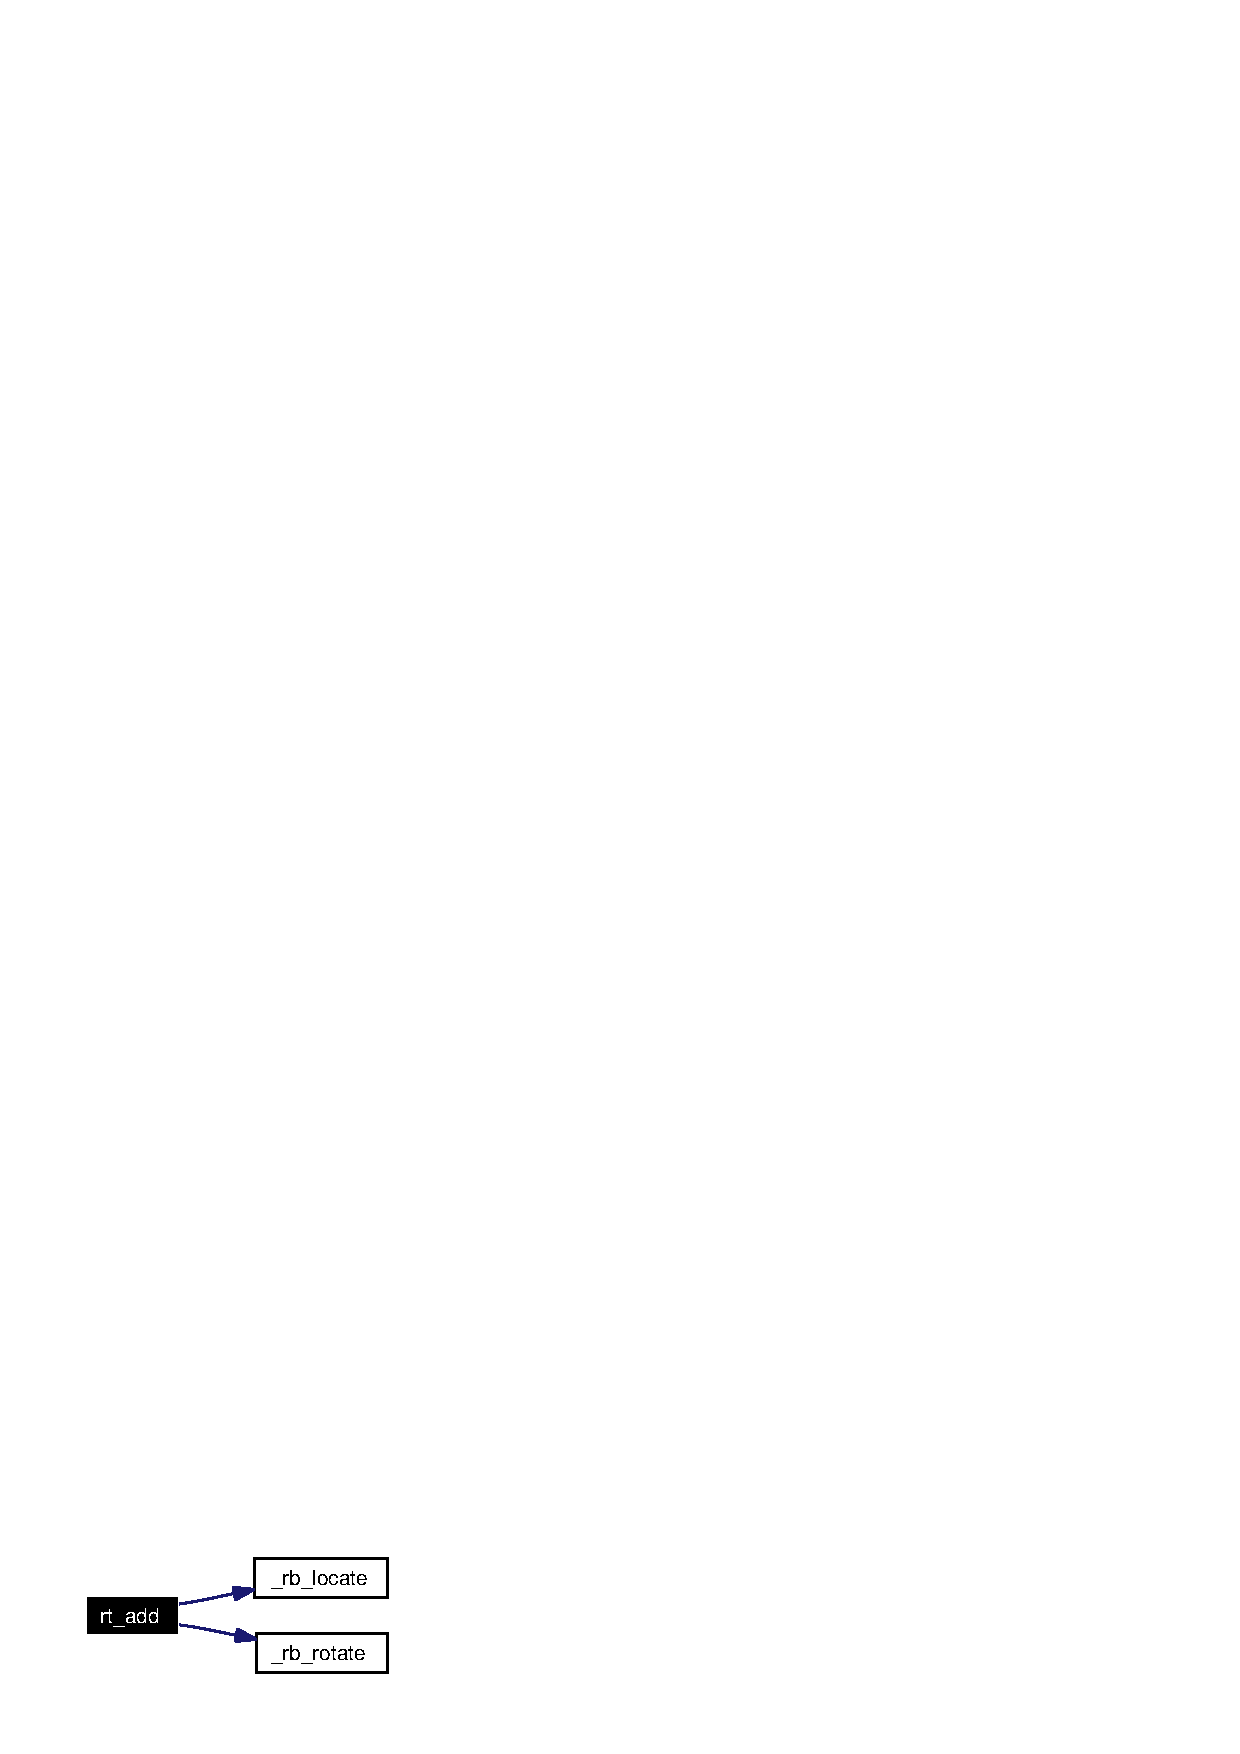
\includegraphics[width=95pt]{group__dbprim__rbtree_ga7_cgraph}
\end{center}
\end{figure}
\hypertarget{group__dbprim__rbtree_ga10}{
\index{dbprim_rbtree@{dbprim\_\-rbtree}!rt_find@{rt\_\-find}}
\index{rt_find@{rt\_\-find}!dbprim_rbtree@{dbprim\_\-rbtree}}
\subsubsection[rt\_\-find]{\setlength{\rightskip}{0pt plus 5cm}unsigned long rt\_\-find (\hyperlink{struct__rb__tree__s}{rb\_\-tree\_\-t} $\ast$ {\em tree}, \hyperlink{struct__rb__node__s}{rb\_\-node\_\-t} $\ast$$\ast$ {\em node\_\-p}, \hyperlink{struct__db__key__s}{db\_\-key\_\-t} $\ast$ {\em key})}}
\label{group__dbprim__rbtree_ga10}


This function looks up an entry matching the given {\tt key}.

\begin{Desc}
\item[Parameters:]
\begin{description}
\item[\mbox{$\leftarrow$} {\em tree}]A pointer to a \hyperlink{group__dbprim__rbtree_ga0}{rb\_\-tree\_\-t}. \item[\mbox{$\rightarrow$} {\em node\_\-p}]A pointer to a pointer to a \hyperlink{group__dbprim__rbtree_ga1}{rb\_\-node\_\-t}. If {\tt NULL} is passed, the lookup will be performed and an appropriate error code returned. \item[\mbox{$\leftarrow$} {\em key}]A pointer to a \hyperlink{group__dbprim_ga0}{db\_\-key\_\-t} describing the item to find.\end{description}
\end{Desc}
\begin{Desc}
\item[Return values:]
\begin{description}
\item[{\em DB\_\-ERR\_\-BADARGS}]An argument was invalid. \item[{\em DB\_\-ERR\_\-NOENTRY}]No matching entry was found.\end{description}
\end{Desc}


Definition at line 34 of file rt\_\-find.c.

References \_\-rb\_\-locate(), \_\-rb\_\-tree\_\-s::rt\_\-count, and rt\_\-verify.

Here is the call graph for this function:\begin{figure}[H]
\begin{center}
\leavevmode
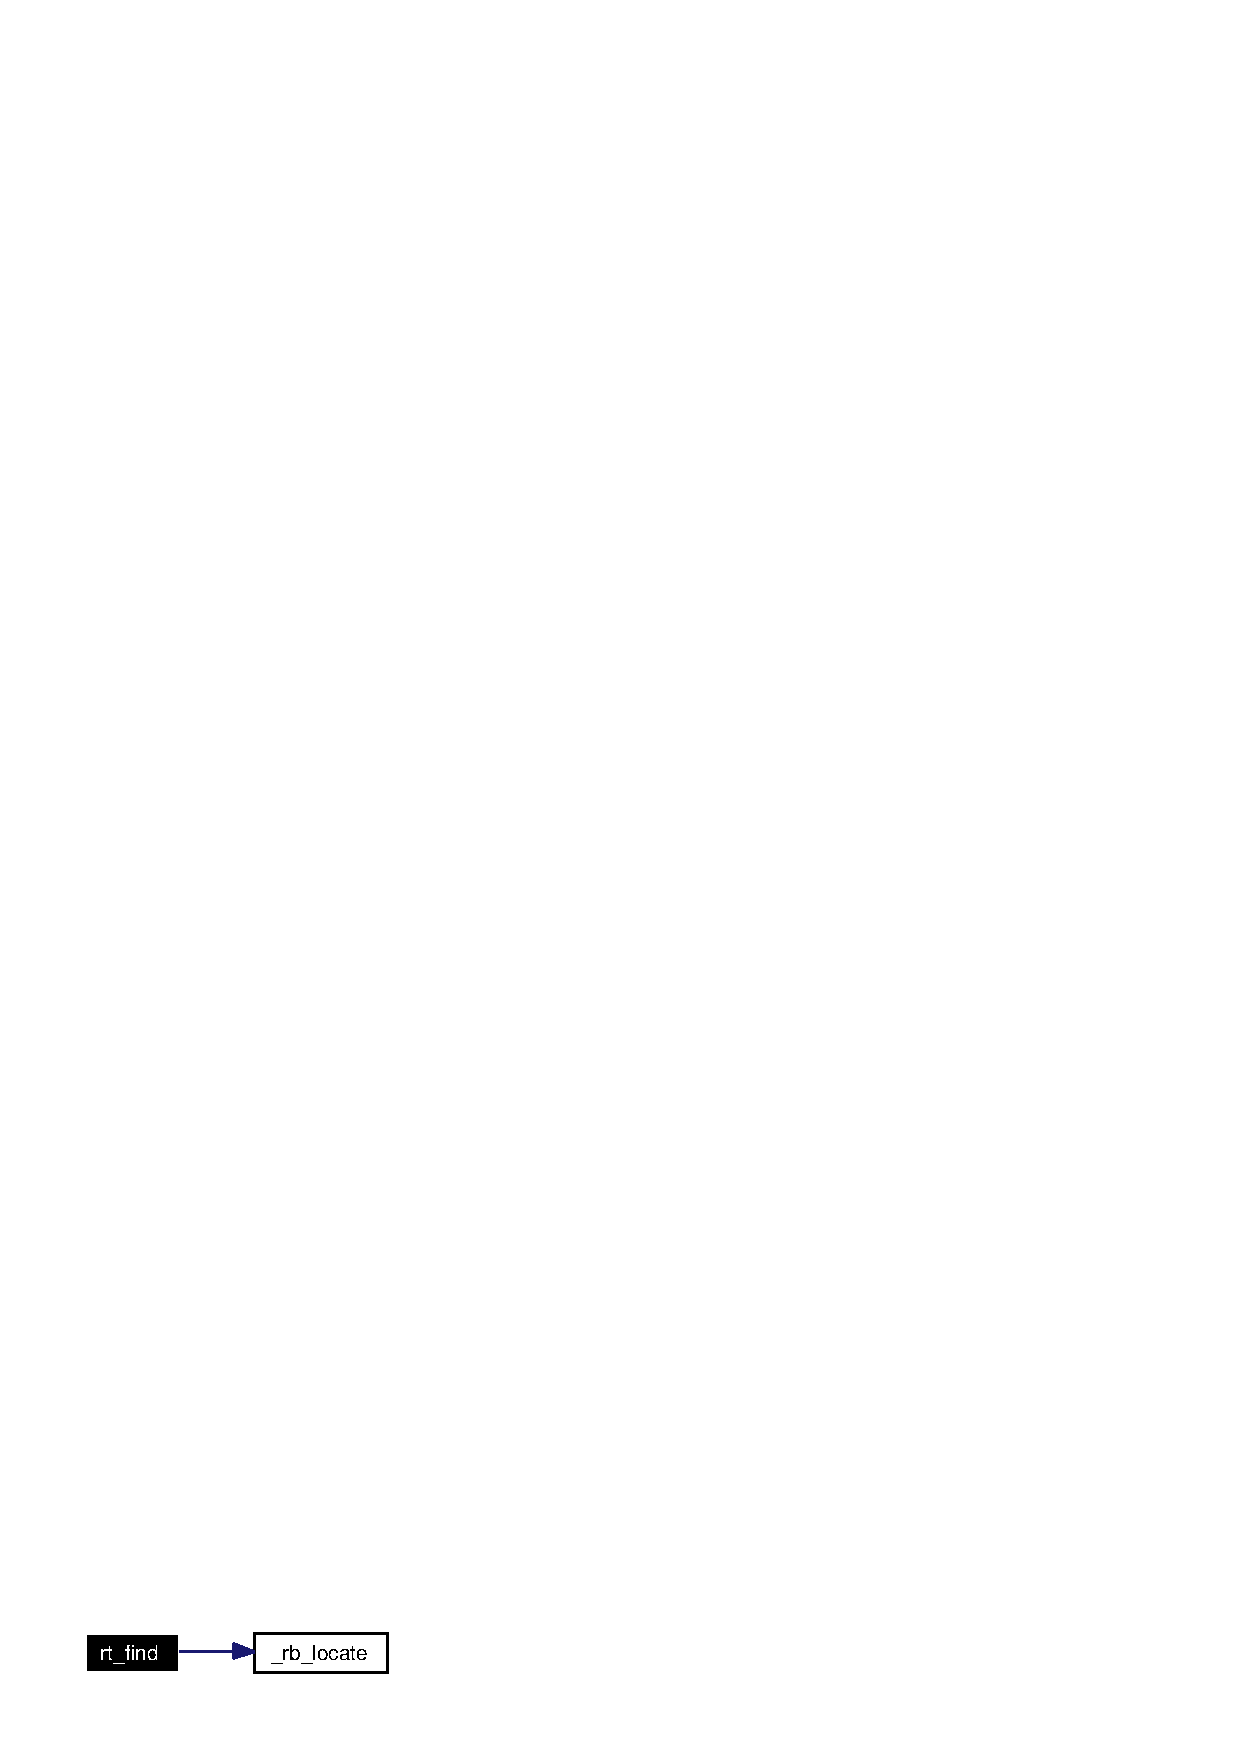
\includegraphics[width=95pt]{group__dbprim__rbtree_ga10_cgraph}
\end{center}
\end{figure}
\hypertarget{group__dbprim__rbtree_ga13}{
\index{dbprim_rbtree@{dbprim\_\-rbtree}!rt_flush@{rt\_\-flush}}
\index{rt_flush@{rt\_\-flush}!dbprim_rbtree@{dbprim\_\-rbtree}}
\subsubsection[rt\_\-flush]{\setlength{\rightskip}{0pt plus 5cm}unsigned long rt\_\-flush (\hyperlink{struct__rb__tree__s}{rb\_\-tree\_\-t} $\ast$ {\em tree}, \hyperlink{group__dbprim__rbtree_ga2}{rb\_\-iter\_\-t} {\em flush\_\-func}, void $\ast$ {\em extra})}}
\label{group__dbprim__rbtree_ga13}


This function flushes a red-black tree--that is, it removes each node from the tree. If a {\tt flush\_\-func} is specified, it will be called on the node after it has been removed from the tree, and may safely call {\tt free()}.

\begin{Desc}
\item[Parameters:]
\begin{description}
\item[\mbox{$\leftarrow$} {\em tree}]A pointer to a \hyperlink{group__dbprim__rbtree_ga0}{rb\_\-tree\_\-t}. \item[\mbox{$\leftarrow$} {\em flush\_\-func}]A pointer to a callback function used to perform user-specified actions on a node after removing it from the tree. May be {\tt NULL}. See the documentation for \hyperlink{group__dbprim__rbtree_ga2}{rb\_\-iter\_\-t} for more information. \item[\mbox{$\leftarrow$} {\em extra}]A {\tt void} pointer that will be passed to {\tt flush\_\-func}.\end{description}
\end{Desc}
\begin{Desc}
\item[Return values:]
\begin{description}
\item[{\em DB\_\-ERR\_\-BADARGS}]An argument was invalid. \item[{\em DB\_\-ERR\_\-FROZEN}]The red-black tree is frozen.\end{description}
\end{Desc}


Definition at line 34 of file rt\_\-flush.c.

References RBT\_\-FLAG\_\-FREEZE, \_\-rb\_\-tree\_\-s::rt\_\-count, \_\-rb\_\-tree\_\-s::rt\_\-flags, rt\_\-remove(), \_\-rb\_\-tree\_\-s::rt\_\-root, and rt\_\-verify.

Here is the call graph for this function:\begin{figure}[H]
\begin{center}
\leavevmode
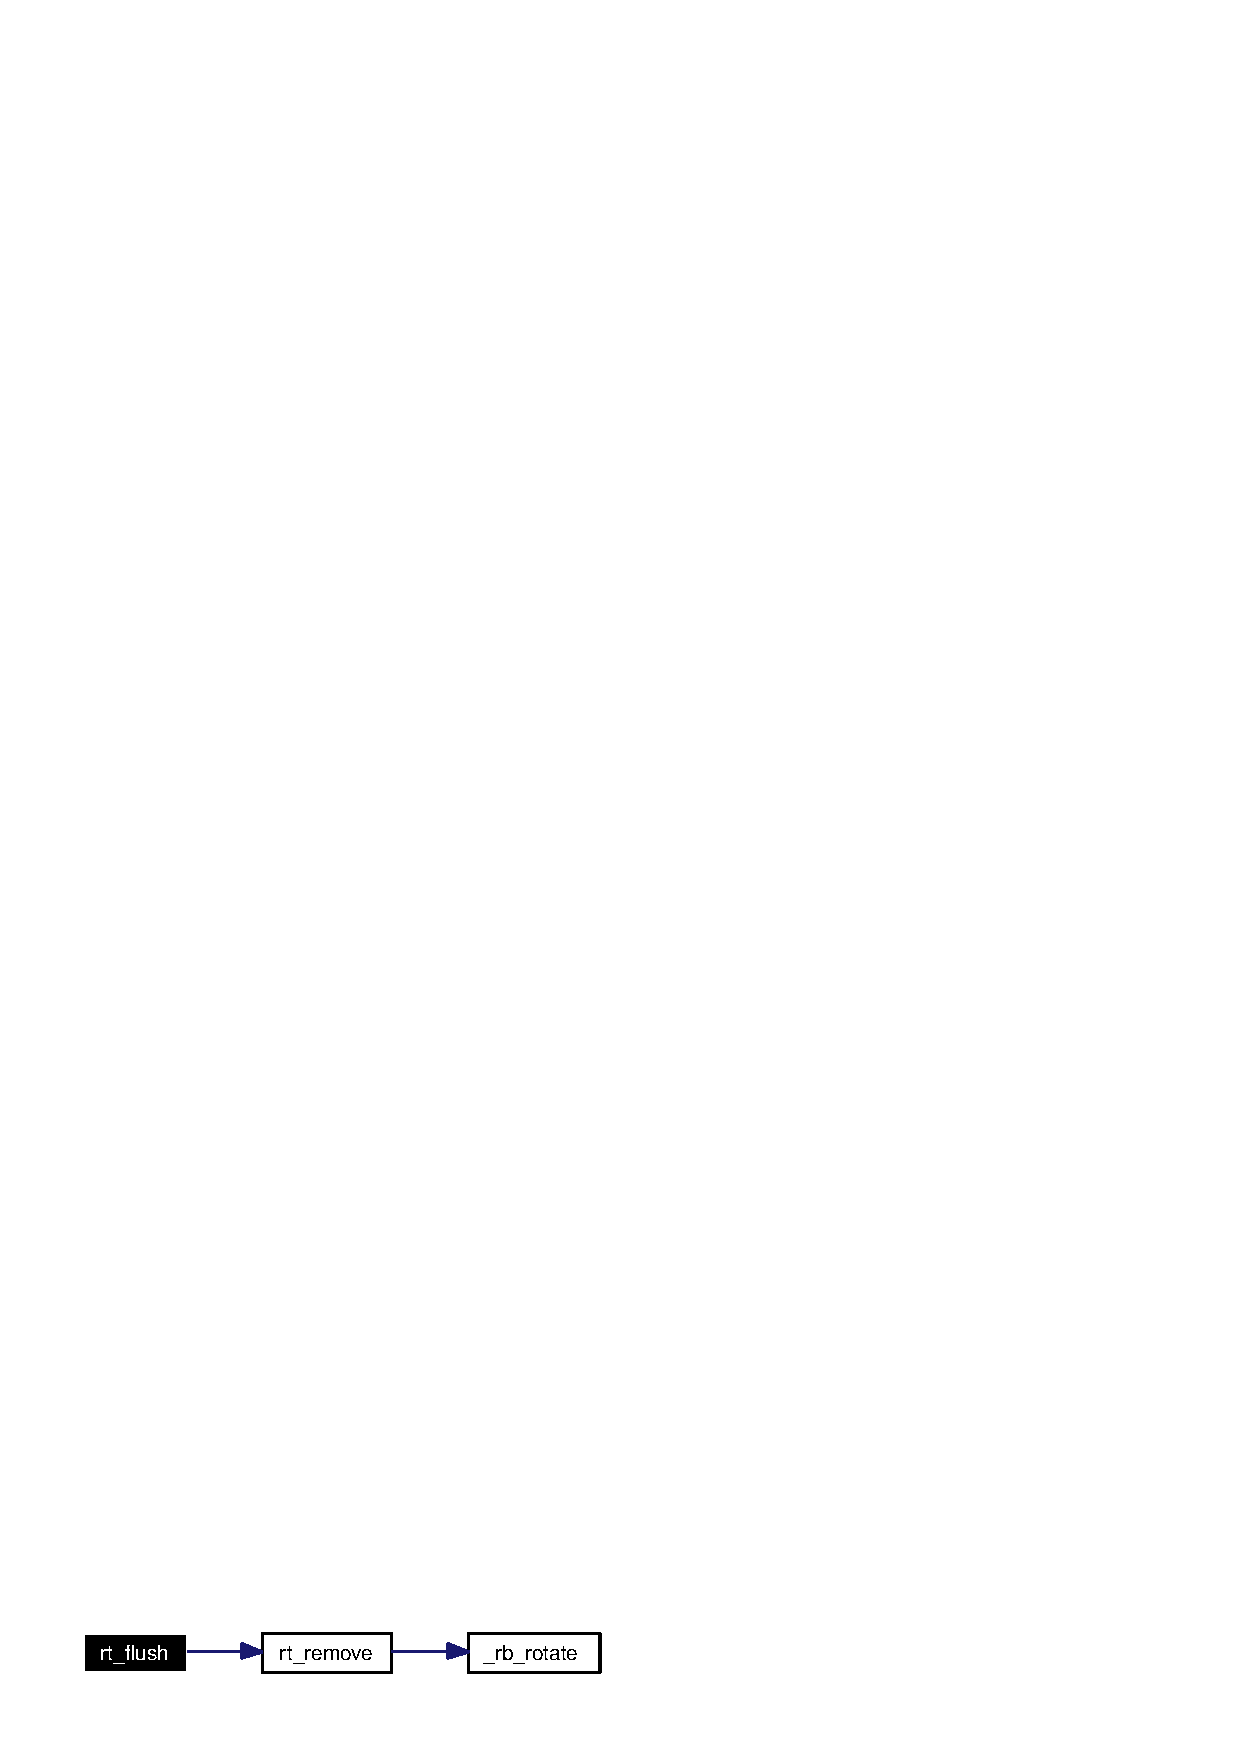
\includegraphics[width=146pt]{group__dbprim__rbtree_ga13_cgraph}
\end{center}
\end{figure}
\hypertarget{group__dbprim__rbtree_ga6}{
\index{dbprim_rbtree@{dbprim\_\-rbtree}!rt_init@{rt\_\-init}}
\index{rt_init@{rt\_\-init}!dbprim_rbtree@{dbprim\_\-rbtree}}
\subsubsection[rt\_\-init]{\setlength{\rightskip}{0pt plus 5cm}unsigned long rt\_\-init (\hyperlink{struct__rb__tree__s}{rb\_\-tree\_\-t} $\ast$ {\em tree}, \hyperlink{group__dbprim__rbtree_ga3}{rb\_\-comp\_\-t} {\em comp}, void $\ast$ {\em extra})}}
\label{group__dbprim__rbtree_ga6}


This function dynamically initializes a red-black tree.

\begin{Desc}
\item[Parameters:]
\begin{description}
\item[\mbox{$\leftarrow$} {\em tree}]A pointer to a \hyperlink{group__dbprim__rbtree_ga0}{rb\_\-tree\_\-t} to be initialized. \item[\mbox{$\leftarrow$} {\em comp}]A \hyperlink{group__dbprim__rbtree_ga3}{rb\_\-comp\_\-t} function pointer for a comparison function. \item[\mbox{$\leftarrow$} {\em extra}]Extra pointer data that should be associated with the tree.\end{description}
\end{Desc}
\begin{Desc}
\item[Return values:]
\begin{description}
\item[{\em DB\_\-ERR\_\-BADARGS}]An invalid argument was given.\end{description}
\end{Desc}


Definition at line 34 of file rt\_\-init.c.

References RB\_\-TREE\_\-MAGIC, \_\-rb\_\-tree\_\-s::rt\_\-comp, \_\-rb\_\-tree\_\-s::rt\_\-count, \_\-rb\_\-tree\_\-s::rt\_\-extra, \_\-rb\_\-tree\_\-s::rt\_\-flags, \_\-rb\_\-tree\_\-s::rt\_\-magic, and \_\-rb\_\-tree\_\-s::rt\_\-root.\hypertarget{group__dbprim__rbtree_ga12}{
\index{dbprim_rbtree@{dbprim\_\-rbtree}!rt_iter@{rt\_\-iter}}
\index{rt_iter@{rt\_\-iter}!dbprim_rbtree@{dbprim\_\-rbtree}}
\subsubsection[rt\_\-iter]{\setlength{\rightskip}{0pt plus 5cm}unsigned long rt\_\-iter (\hyperlink{struct__rb__tree__s}{rb\_\-tree\_\-t} $\ast$ {\em tree}, \hyperlink{struct__rb__node__s}{rb\_\-node\_\-t} $\ast$ {\em start}, \hyperlink{group__dbprim__rbtree_ga2}{rb\_\-iter\_\-t} {\em iter\_\-func}, void $\ast$ {\em extra}, unsigned long {\em flags})}}
\label{group__dbprim__rbtree_ga12}


This function iterates over every node in a red-black tree in the given traversal order, executing the given {\tt iter\_\-func} on each node.

\begin{Desc}
\item[Parameters:]
\begin{description}
\item[\mbox{$\leftarrow$} {\em tree}]A pointer to a \hyperlink{group__dbprim__rbtree_ga0}{rb\_\-tree\_\-t}. \item[\mbox{$\leftarrow$} {\em start}]A pointer to a \hyperlink{group__dbprim__rbtree_ga1}{rb\_\-node\_\-t} describing where in the tree to start. If {\tt NULL} is passed, the first element of the tree for the specified order will be assumed. \item[\mbox{$\leftarrow$} {\em iter\_\-func}]A pointer to a callback function used to perform user-specified actions on a node in the red-black tree. {\tt NULL} is an invalid value. See the documentation for \hyperlink{group__dbprim__rbtree_ga2}{rb\_\-iter\_\-t} for more information. \item[\mbox{$\leftarrow$} {\em extra}]A {\tt void} pointer that will be passed to {\tt iter\_\-func}. \item[\mbox{$\leftarrow$} {\em flags}]One of RBT\_\-ORDER\_\-PRE, RBT\_\-ORDER\_\-IN, or RBT\_\-ORDER\_\-POST, possibly ORed with DB\_\-FLAG\_\-REVERSE to reverse the order of iteration. Zero is not allowed.\end{description}
\end{Desc}
\begin{Desc}
\item[Return values:]
\begin{description}
\item[{\em DB\_\-ERR\_\-BADARGS}]An argument was invalid. \item[{\em DB\_\-ERR\_\-WRONGTABLE}]{\tt start} is not in this red-black tree.\end{description}
\end{Desc}


Definition at line 34 of file rt\_\-iter.c.

References RBT\_\-FLAG\_\-FREEZE, RBT\_\-ORDER\_\-MASK, \_\-rb\_\-node\_\-s::rn\_\-tree, rn\_\-verify, \_\-rb\_\-tree\_\-s::rt\_\-flags, rt\_\-next(), and rt\_\-verify.

Here is the call graph for this function:\begin{figure}[H]
\begin{center}
\leavevmode
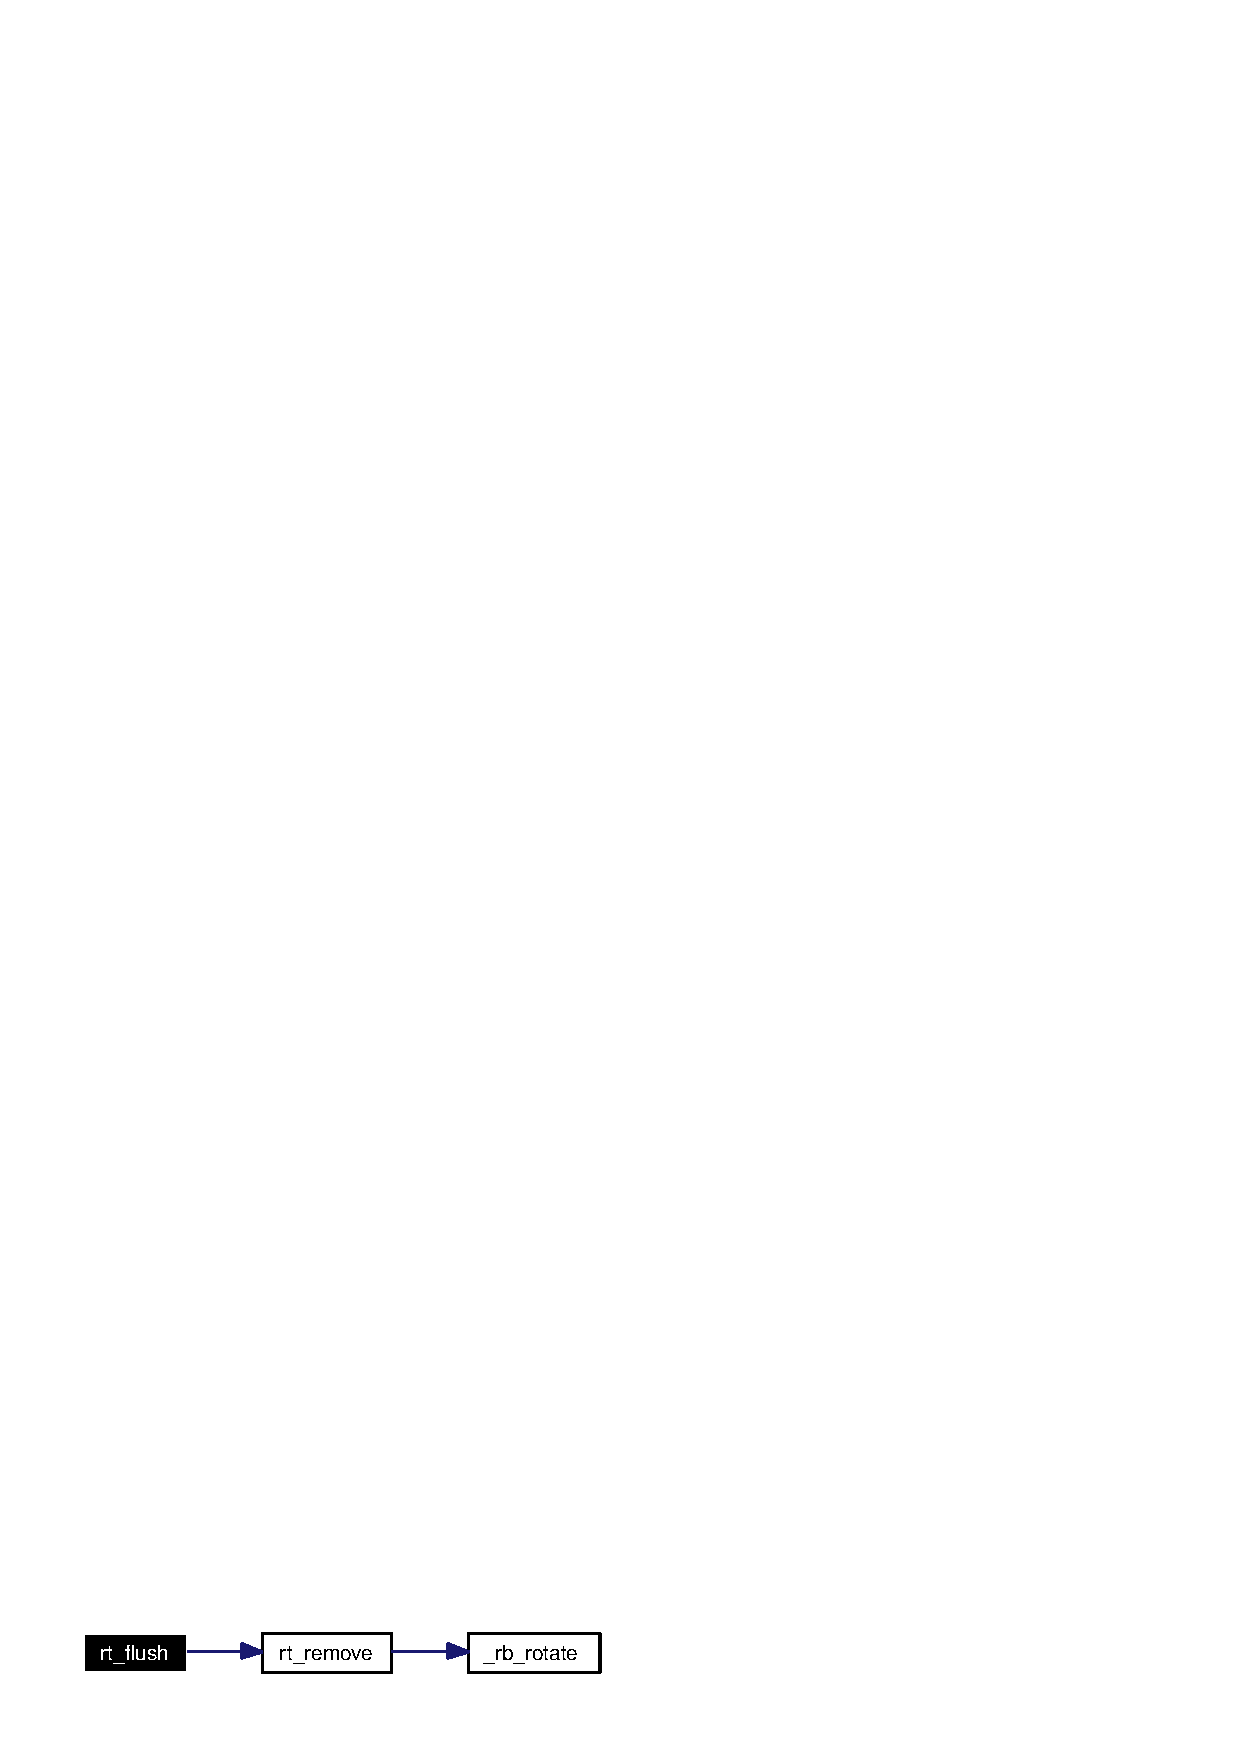
\includegraphics[width=85pt]{group__dbprim__rbtree_ga12_cgraph}
\end{center}
\end{figure}
\hypertarget{group__dbprim__rbtree_ga8}{
\index{dbprim_rbtree@{dbprim\_\-rbtree}!rt_move@{rt\_\-move}}
\index{rt_move@{rt\_\-move}!dbprim_rbtree@{dbprim\_\-rbtree}}
\subsubsection[rt\_\-move]{\setlength{\rightskip}{0pt plus 5cm}unsigned long rt\_\-move (\hyperlink{struct__rb__tree__s}{rb\_\-tree\_\-t} $\ast$ {\em tree}, \hyperlink{struct__rb__node__s}{rb\_\-node\_\-t} $\ast$ {\em node}, \hyperlink{struct__db__key__s}{db\_\-key\_\-t} $\ast$ {\em key})}}
\label{group__dbprim__rbtree_ga8}


This function moves an existing node in the red-black tree to correspond to the new key.

\begin{Desc}
\item[Parameters:]
\begin{description}
\item[\mbox{$\leftarrow$} {\em tree}]A pointer to a \hyperlink{group__dbprim__rbtree_ga0}{rb\_\-tree\_\-t}. \item[\mbox{$\leftarrow$} {\em node}]A pointer to a \hyperlink{group__dbprim__rbtree_ga1}{rb\_\-node\_\-t} to be moved. It must already be in the red-black tree. \item[\mbox{$\leftarrow$} {\em key}]A pointer to a \hyperlink{group__dbprim_ga0}{db\_\-key\_\-t} describing the new key for the node.\end{description}
\end{Desc}
\begin{Desc}
\item[Return values:]
\begin{description}
\item[{\em DB\_\-ERR\_\-BADARGS}]An invalid argument was given. \item[{\em DB\_\-ERR\_\-UNUSED}]Node is not in a red-black tree. \item[{\em DB\_\-ERR\_\-WRONGTABLE}]Node is not in this tree. \item[{\em DB\_\-ERR\_\-FROZEN}]Red-black tree is frozen. \item[{\em DB\_\-ERR\_\-DUPLICATE}]New key is a duplicate of an existing key. \item[{\em DB\_\-ERR\_\-READDFAILED}]Unable to re-add node to tree.\end{description}
\end{Desc}


Definition at line 35 of file rt\_\-move.c.

References \_\-rb\_\-locate(), RBT\_\-FLAG\_\-FREEZE, \_\-rb\_\-node\_\-s::rn\_\-tree, rn\_\-verify, rt\_\-add(), \_\-rb\_\-tree\_\-s::rt\_\-flags, rt\_\-remove(), and rt\_\-verify.

Here is the call graph for this function:\begin{figure}[H]
\begin{center}
\leavevmode
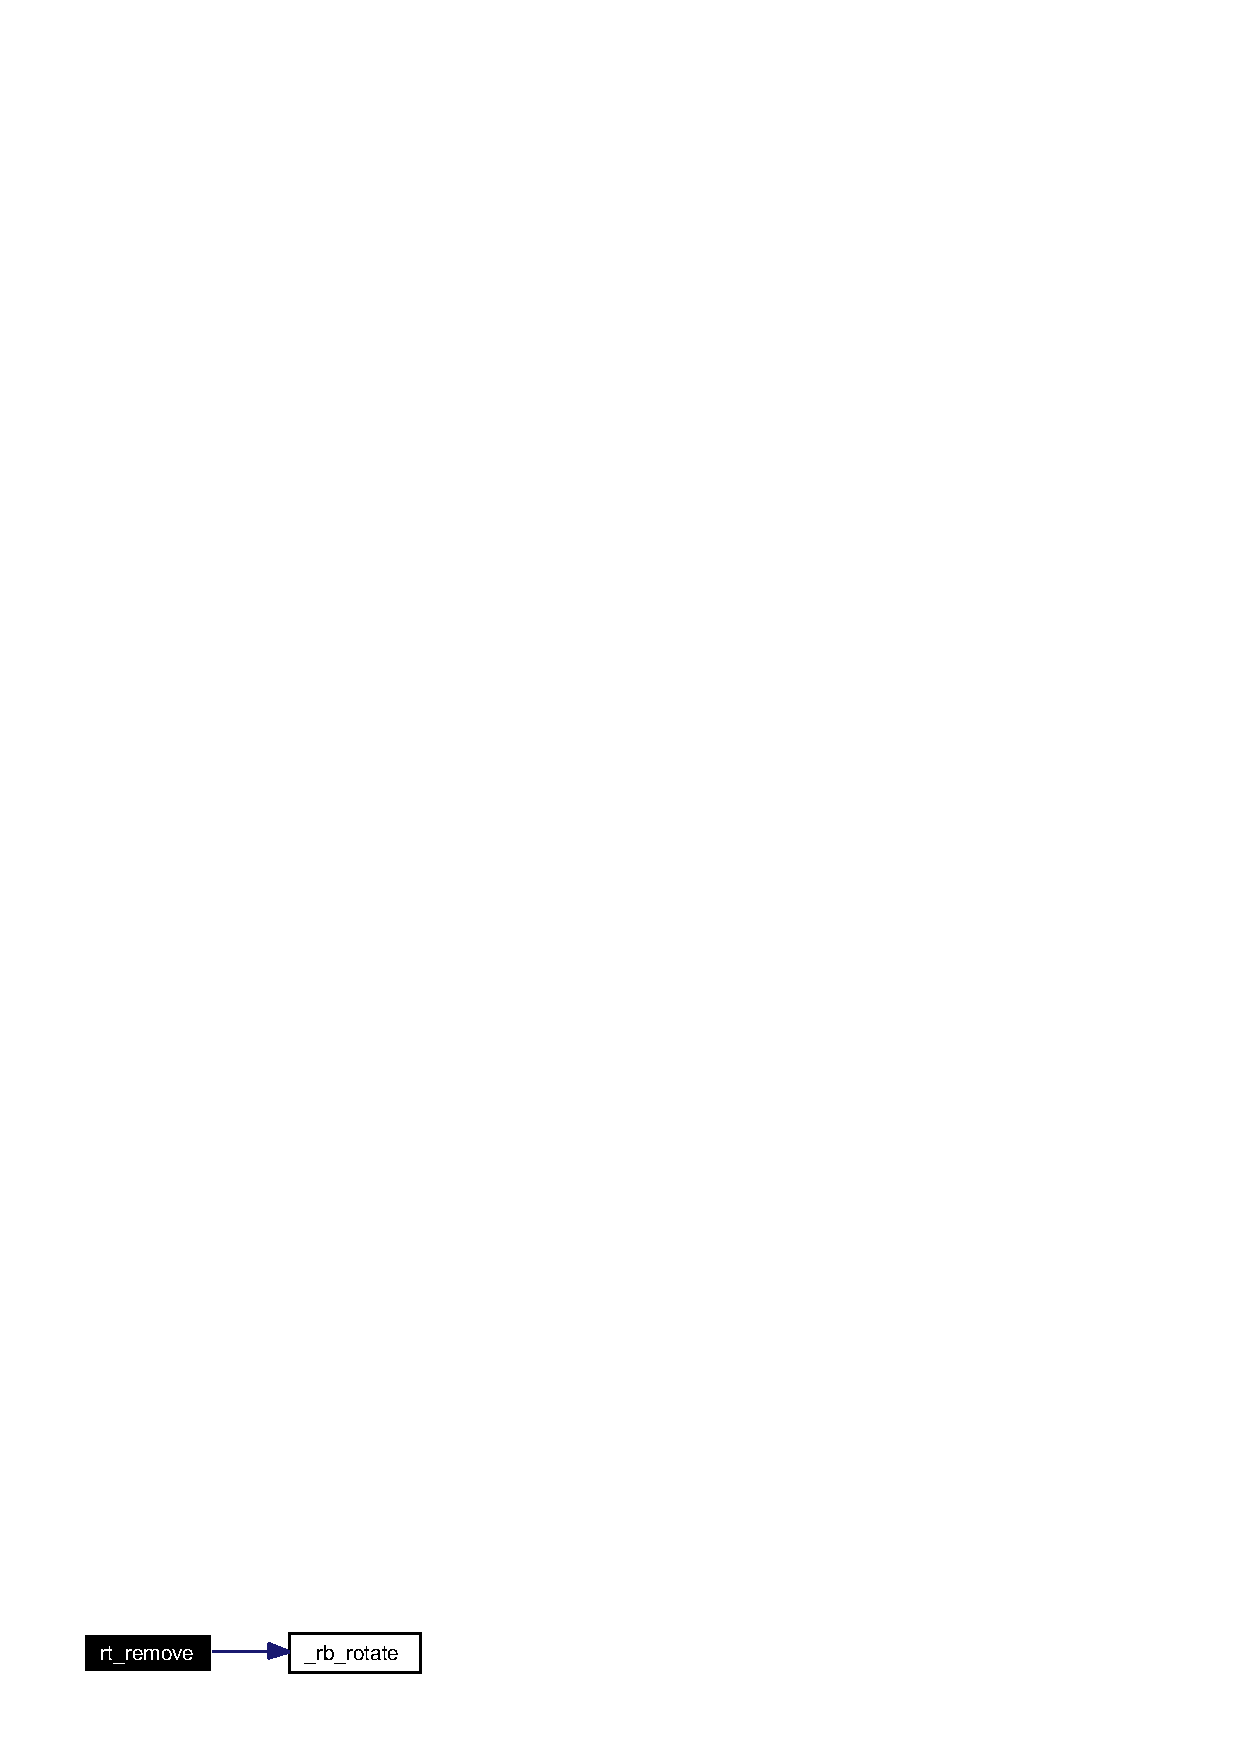
\includegraphics[width=148pt]{group__dbprim__rbtree_ga8_cgraph}
\end{center}
\end{figure}
\hypertarget{group__dbprim__rbtree_ga11}{
\index{dbprim_rbtree@{dbprim\_\-rbtree}!rt_next@{rt\_\-next}}
\index{rt_next@{rt\_\-next}!dbprim_rbtree@{dbprim\_\-rbtree}}
\subsubsection[rt\_\-next]{\setlength{\rightskip}{0pt plus 5cm}unsigned long rt\_\-next (\hyperlink{struct__rb__tree__s}{rb\_\-tree\_\-t} $\ast$ {\em tree}, \hyperlink{struct__rb__node__s}{rb\_\-node\_\-t} $\ast$$\ast$ {\em node\_\-io}, unsigned long {\em flags})}}
\label{group__dbprim__rbtree_ga11}


This function obtains the next node in the given iteration scheme. The {\tt node\_\-io} parameter is a value-result parameter--if the node pointer to which it points is {\tt NULL}, the first node for the given iteration order will be loaded; otherwise, the next node in the given iteration order will be loaded.

\begin{Desc}
\item[Parameters:]
\begin{description}
\item[\mbox{$\leftarrow$} {\em tree}]A pointer to a \hyperlink{group__dbprim__rbtree_ga0}{rb\_\-tree\_\-t}. \item[\mbox{$\leftrightarrow$} {\em node\_\-io}]A pointer to a pointer to a \hyperlink{group__dbprim__rbtree_ga1}{rb\_\-node\_\-t}. If the pointer to which node\_\-io points is {\tt NULL}, the first node will be loaded, otherwise the next node will be loaded. \item[\mbox{$\leftarrow$} {\em flags}]One of RBT\_\-ORDER\_\-PRE, RBT\_\-ORDER\_\-IN, or RBT\_\-ORDER\_\-POST, possibly ORed with DB\_\-FLAG\_\-REVERSE to reverse the order of iteration. Zero is not allowed.\end{description}
\end{Desc}
\begin{Desc}
\item[Return values:]
\begin{description}
\item[{\em DB\_\-ERR\_\-BADARGS}]An argument was invalid. \item[{\em DB\_\-ERR\_\-WRONGTABLE}]{\tt start} is not in this red-black tree.\end{description}
\end{Desc}


Definition at line 34 of file rt\_\-next.c.

References DB\_\-FLAG\_\-REVERSE, RBT\_\-ORDER\_\-IN, RBT\_\-ORDER\_\-MASK, RBT\_\-ORDER\_\-POST, RBT\_\-ORDER\_\-PRE, rn\_\-isleft, rn\_\-isright, \_\-rb\_\-node\_\-s::rn\_\-left, \_\-rb\_\-node\_\-s::rn\_\-parent, \_\-rb\_\-node\_\-s::rn\_\-right, \_\-rb\_\-node\_\-s::rn\_\-tree, rn\_\-verify, \_\-rb\_\-tree\_\-s::rt\_\-root, and rt\_\-verify.

Referenced by rt\_\-iter().\hypertarget{group__dbprim__rbtree_ga9}{
\index{dbprim_rbtree@{dbprim\_\-rbtree}!rt_remove@{rt\_\-remove}}
\index{rt_remove@{rt\_\-remove}!dbprim_rbtree@{dbprim\_\-rbtree}}
\subsubsection[rt\_\-remove]{\setlength{\rightskip}{0pt plus 5cm}unsigned long rt\_\-remove (\hyperlink{struct__rb__tree__s}{rb\_\-tree\_\-t} $\ast$ {\em tree}, \hyperlink{struct__rb__node__s}{rb\_\-node\_\-t} $\ast$ {\em node})}}
\label{group__dbprim__rbtree_ga9}


This function removes the given node from the specified red-black tree.

\begin{Desc}
\item[Parameters:]
\begin{description}
\item[\mbox{$\leftarrow$} {\em tree}]A pointer to a \hyperlink{group__dbprim__rbtree_ga0}{rb\_\-tree\_\-t}. \item[\mbox{$\leftarrow$} {\em node}]A pointer to a \hyperlink{group__dbprim__rbtree_ga1}{rb\_\-node\_\-t} to be removed from the tree.\end{description}
\end{Desc}
\begin{Desc}
\item[Return values:]
\begin{description}
\item[{\em DB\_\-ERR\_\-BADARGS}]An invalid argument was given. \item[{\em DB\_\-ERR\_\-UNUSED}]Node is not in a red-black tree. \item[{\em DB\_\-ERR\_\-WRONGTABLE}]Node is not in this tree. \item[{\em DB\_\-ERR\_\-FROZEN}]Red-black tree is frozen.\end{description}
\end{Desc}


Definition at line 154 of file rt\_\-remove.c.

References \_\-rb\_\-rotate(), \_\-rn\_\-clear, \_\-rt\_\-update\_\-parent, l\_\-neph, r\_\-neph, RB\_\-COLOR\_\-BLACK, RB\_\-COLOR\_\-RED, RBT\_\-FLAG\_\-FREEZE, \_\-rb\_\-node\_\-s::rn\_\-color, rn\_\-isblack, rn\_\-isred, \_\-rb\_\-node\_\-s::rn\_\-left, \_\-rb\_\-node\_\-s::rn\_\-parent, \_\-rb\_\-node\_\-s::rn\_\-right, \_\-rb\_\-node\_\-s::rn\_\-tree, rn\_\-verify, \_\-rb\_\-tree\_\-s::rt\_\-count, \_\-rb\_\-tree\_\-s::rt\_\-flags, \_\-rb\_\-tree\_\-s::rt\_\-root, rt\_\-verify, and sibling.

Referenced by rt\_\-flush(), and rt\_\-move().

Here is the call graph for this function:\begin{figure}[H]
\begin{center}
\leavevmode
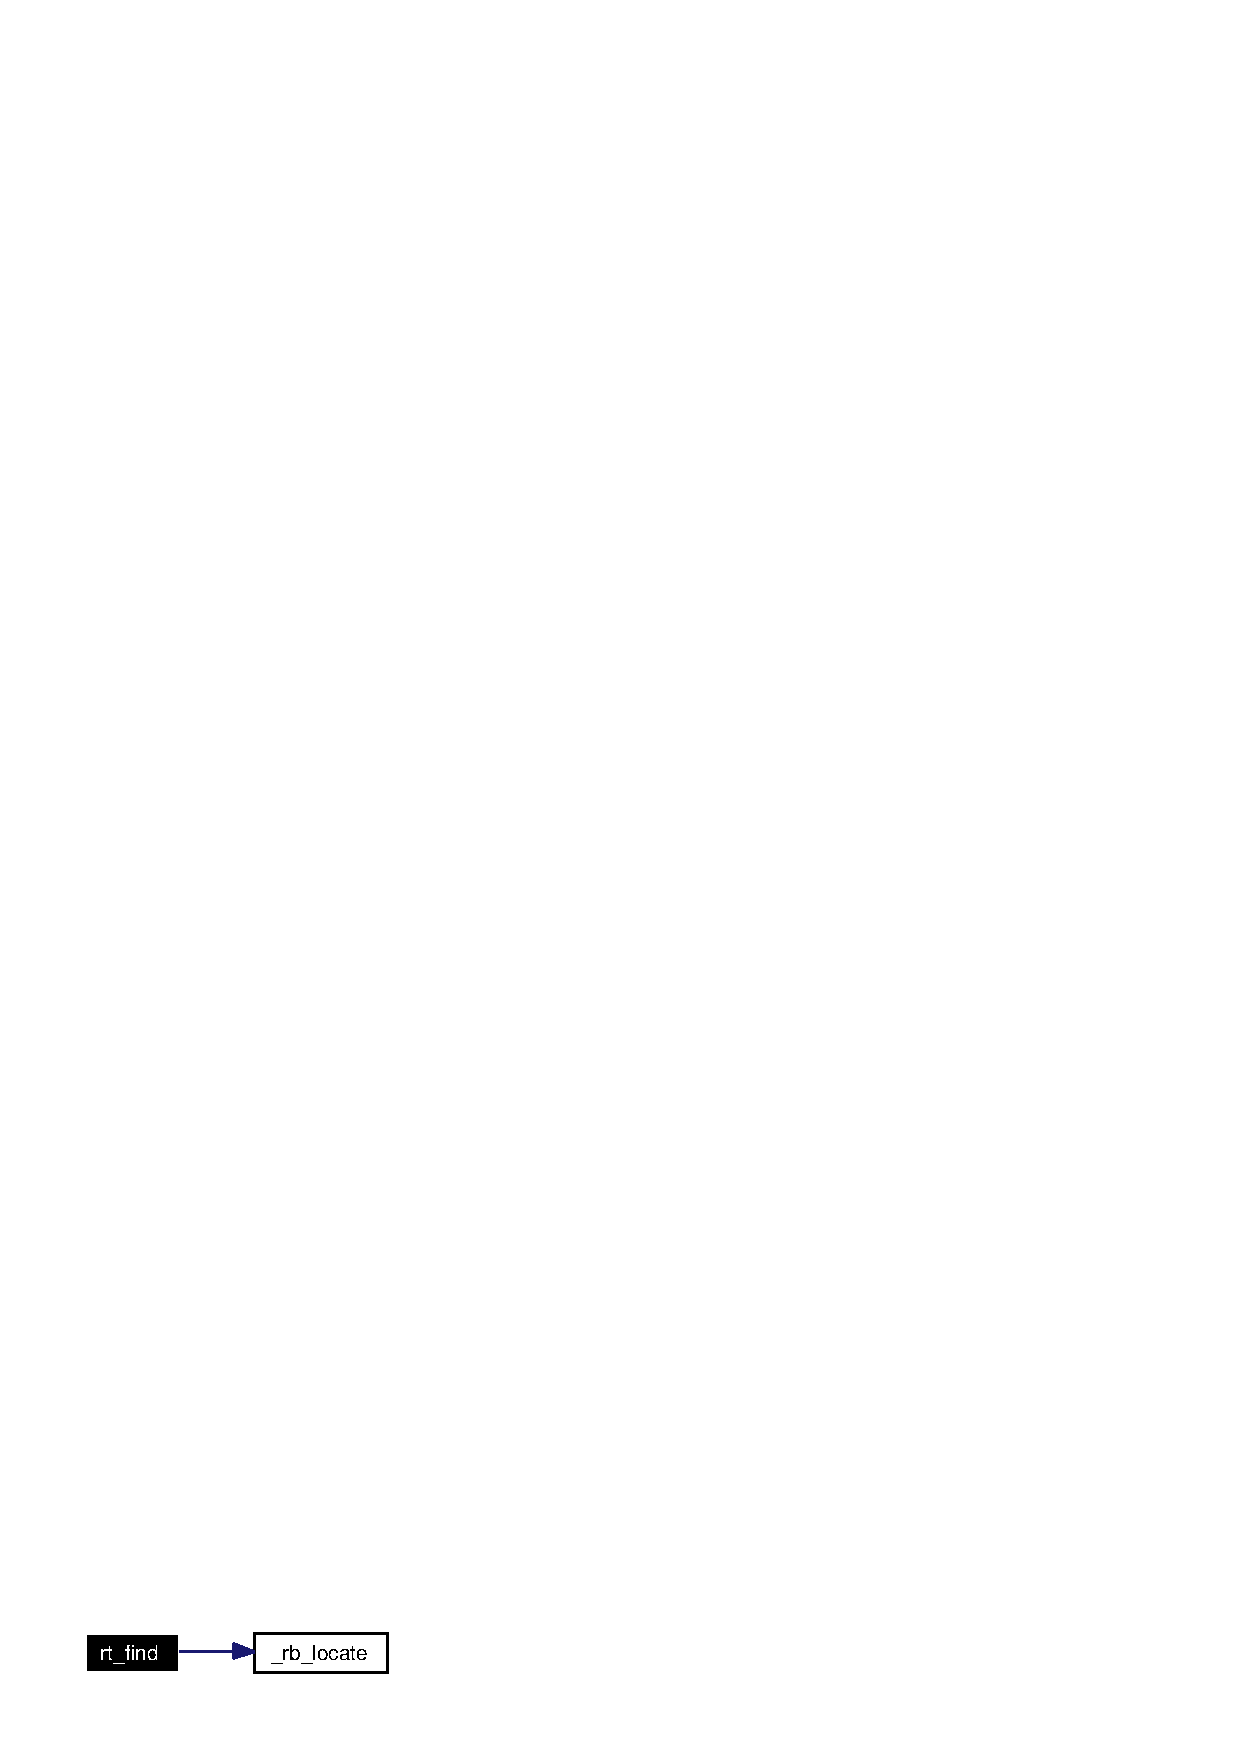
\includegraphics[width=103pt]{group__dbprim__rbtree_ga9_cgraph}
\end{center}
\end{figure}
